%\def\R{$\textsf{R}$}
%\def\S{$\textsf{S}$}

%\renewcommand{\labelitemii}{$\circ$}
\newcommand{\sfa}{a}
\newcommand{\worst}{\mbox{\em worst}}
\newcommand{\best}{\mbox{\em best}}
\newcommand{\regret}{\mbox{\em regret}}
\newcommand{\opt}{\mbox{\em opt}}
\newcommand{\join}{\bowtie}
\newcommand{\lE}{\underline{E}}
\newcommand{\uE}{\overline{E}}
\newcommand{\heads}{{\it heads}}
\newcommand{\tails}{{\it tails}}

\newcommand{\A}{{\cal A}}
\newcommand{\B}{{\cal B}}
\newcommand{\C}{{\cal C}}
\newcommand{\D}{{\cal D}}
\newcommand{\E}{{\cal E}}
\newcommand{\F}{{\cal F}}
\newcommand{\G}{{\cal G}}
%\newcommand{\H}{{\cal H}}
\newcommand{\I}{{\cal I}}
\newcommand{\J}{{\cal J}}
\newcommand{\K}{{\cal K}}
%\newcommand{\L}{{\cal L}}
\newcommand{\M}{{\cal M}}
\newcommand{\N}{{\cal N}}
%\newcommand{\O}{{\cal O}}
\newcommand{\Ocal}{{\cal O}}
\newcommand{\Hcal}{{\cal H}}
\renewcommand{\P}{{\cal P}}
\newcommand{\Q}{{\cal Q}}
\newcommand{\R}{{\cal R}}
%\newcommand{\S}{{\cal S}}
\newcommand{\T}{{\cal T}}
\newcommand{\U}{{\cal U}}
\newcommand{\V}{{\cal V}}
\newcommand{\W}{{\cal W}}
\newcommand{\X}{{\cal X}}
\newcommand{\Y}{{\cal Y}}
\newcommand{\Z}{{\cal Z}}


\newcommand{\IR}{\mathbb{R}}
\newcommand{\dfn}{\begin{definition}}
\newcommand{\edfn}{\end{definition}}
\newcommand{\thm}{\begin{theorem}}
\newcommand{\ethm}{\end{theorem}}
\newcommand{\xam}{\begin{example}}
\newcommand{\exam}{\end{example}}
\newcommand{\inter}{\cap}
\newcommand{\union}{\cup}




\documentclass[t, 8pt, seriff]{beamer}


%\documentclass[a4paper,xcolor=svgnames]{beamer} 
\usepackage[portuguese]{babel}
\usepackage[utf8]{inputenc}
\usepackage{times}
\usepackage{amsmath,amsthm}
\usepackage{amssymb,latexsym}
\usepackage{graphics}
%\usepackage{graphicx}

\usepackage{multimedia}
% \usepackage{movie15}
\usepackage{media9}

\usetheme{default}
%\usetheme{Singapore}
%\usetheme{PaloAlto} 
\usetheme{Boadilla}
% other themes: AnnArbor, Antibes, Bergen, Berkeley, Berlin, Boadilla, boxes, CambridgeUS, Copenhagen, Darmstadt, default, Dresden, Frankfurt, Goettingen,
% Hannover, Ilmenau, JuanLesPins, Luebeck, Madrid, Maloe, Marburg, Montpellier, PaloAlto, Pittsburg, Rochester, Singapore, Szeged, boxes, default

\useoutertheme{infolines}
%\usefonttheme{serif}
% you can also specify font themes: default, professionalfonts, serif, structurebold, structureitalicserif, structuresmallcapsserif

%\definecolor{vermelho}{RGB}{100,30,40}
%\definecolor{vermelholys}{RGB}{132,158,139}
%\definecolor{vermelholyslys}{RGB}{173,190,177}
%\definecolor{vermelholyslyslys}{RGB}{214,223,216}


%\usecolortheme[named=vermelho]{structure}




 



%\documentclass[a4paper,xcolor=svgnames]{beamer} 
%\usepackage[brazil]{babel}
%\usepackage[latin1]{inputenc}
\usepackage{ragged2e}
\usepackage{bm}
\usepackage[T1]{fontenc}
%\usepackage{amsmath,amsthm,amsfonts,amssymb} 
\usepackage{multirow}
%\usetheme{CambridgeUS} 
%\setbeamercolor{normal text}{bg=white}
\usepackage {graphicx,color}

\usepackage{wrapfig} % inserir a figura ao lado do texto
\usepackage[dvips]{epsfig} % inserir figuras de extensao post script (ps)
\usepackage{textcomp}
% \usepackage{undertilde} % colocar o til abaixo do x
\usepackage{multicol} % cor na linha
\usepackage{tabularx}
\usepackage{rotating} %rotacionar figuras e tabelas


\usepackage{ragged2e}
%\justifying



\newtheorem{lema}{Lema}
\newtheorem{defi}{Definição}
\newtheorem{teo}{Teorema}
\newtheorem{corol}{Corolário}
\newtheorem{prop}{Proposição}


\newtheoremstyle{Exercício}{}{}{\rm}{}{\bf $\bigstar$ }{:}{ }{} %% \scshape para mudar
\theoremstyle{Exercício}
\newtheorem{exer}{Exercício}

\theoremstyle{plain}
\newtheoremstyle{Exemplo}{}{}{\rm}{}{\bf $\rhd$ }{:}{ }{} %% \scshape para mudar
%o tamanho a maiusculo
\theoremstyle{Exemplo}
\newtheorem{exem}{Exemplo}

% 
% \theoremstyle{plain}
% \newtheoremstyle{Nota}{}{}{\rm}{}{\bf\scshape}{:}{ }{}
% \theoremstyle{Nota}
 \newtheorem{nota}{Nota}






%\setlength{\rightskip}{0pt}
%\setlength{\leftskip}{0pt}
%\setlength{\spaceskip}{0pt}
%\setlength{\xspaceskip}{0pt}



\newcommand{\fullpage}[1]{
\begin{frame}
 #1
\end{frame}
}


\setbeamersize{text margin left=3em, text margin right=3em}



\setbeamertemplate{theorems}[numbered]



\definecolor{links}{HTML}{2A1B81}
\hypersetup{colorlinks,linkcolor=,urlcolor=links}


\graphicspath{{./graphics/}} 			% path das figuras (recomendável)

\newcommand{\cor}[1]{ \{{#1}\}}


\title[Probabilidade]{  Probabilidade (PGE950) }
\author[ Raydonal Ospina  \& Leandro  Rêgo
%\textcopyright 
\ ]{
%Probabilidade\\ 
% Sessão 1 \\
${}$ \\
Raydonal Ospina  \& Leandro  Rêgo }

\date[PGE950 2018-I]{{\tiny PGE950 2018-I}}

\institute[UFPE]{Departamento de Estatística\\
Universidade Federal de Pernambuco\\
Recife/PE}


\usecolortheme[rgb={0,0.3,0.5}]{structure}


%%%%%%%%%%%%%%%%%%%%%%%%%%%%%%%%%%%%%%%%%%%%%%%%%%%%%%%%%%%%%%%%%%%%%%
\begin{document}
% \SweaveOpts{concordance=TRUE}
\begin{frame}
  \titlepage
\end{frame}
%%%%%%%%%%%%%%%%%%%%%%%%%%%%%%%%%%%%%%%%%%%%%%%%%%%%%%%%%%%%%%%%%%%%%%


%=====================================================================

\begin{frame}
\frametitle{Revisão de teoria de conjuntos}

Um {\it conjunto} representa uma coleção de objetos geralmente representado pelas letras maiúsculas, $A,$ $B,$ etc.
\begin{exem} 
\begin{itemize}
\item O conjunto cujos elementos são as vogais $a, e, i, o$ e $u,$ i.e. $$A=\{ a, e, i, o, u\}.$$ 
\item O conjunto de dias da semana $$A=\{ \text{segunda, terça, quarta, quinta, sesta, sábado, domingo} \}.$$ 
\item O conjunto de números inteiros. $A=\mathbb{Z}= \{ 1,2, \ldots \}.$ 
\item O conjunto de números reais.  $A=\mathbb{R}.$ 
\item O conjunto de soluções da equação quadrática $x^2-x-2=0,$  $A=\{ -1, 2 \}.$ 
\end{itemize}
\end{exem} 
$\bullet$ Se $A \,$ e $B \,$ são conjuntos e todo elemento $ x$ pertencente a $A$ também pertence a $B$ então o conjunto $A$ é dito um subconjunto do conjunto $B$ denotado por $A \subseteq B$. Esta definição inclui o caso em que $A$ e $B$ possuem os mesmos elementos, isto é, são o mesmo conjunto $(A = B)$.

$\bullet$ O conjunto que contem todos os conjuntos considerados é denominado de  {\it universo} $\Omega.$


\end{frame}
%=====================================================================


%=====================================================================
\begin{frame}

\begin{block}{Operações entre conjuntos}
Se $A$ e $B$ são eventos, as operações de união, interseção, diferença e complemento entre conjuntos (operações que geram novos conjuntos) são denotadas respectivamente por $A \cup B,$   $A\cap B,$ $A \setminus B$ e $A^\complement.$ As anteriores operações indicam: 
\begin{itemize}
 \item $A\cup B = \{ \omega: \omega\in A \quad \text{ou} \quad \omega\in B\}$ é
um evento que acontece, se e somente se, $A$ ou $B$ acontecem.
\item $A\cap B =\{ \omega: \omega\in A \quad  \text{e} \quad \omega\in B\}$ é um
evento que acontece, se e somente se, $A$ e $B$ acontecem.
\item $A -  B$ é o evento que acontece, se e somente se, $A$ acontece, mas $B$ não acontece.
\item $A^\complement =\{ \omega\in \Omega: \omega\notin A\}$ é o evento que acontece, se e somente se, $A$ não acontece.

\item Dois conjuntos $A$ e $B$, são ditos disjuntos (ou excludentes) se: $A\cap B = \emptyset\,$
\item Uma família de conjuntos é dita disjunta dois a dois ou mutuamente disjunta se dados dois conjuntos quaisquer da família, eles são disjuntos. Mais formalmente falando, seja $A_\lambda $, uma família de conjuntos disjuntos indexados pelo índice $\lambda\in\Lambda\,$ então:
$$
A_i\cap A_j=\emptyset,~~\forall i,j\in\Lambda,~i\neq j\,
$$
\end{itemize}
\end{block}
Note que $ \bigcap_{\lambda\in\Lambda} A_\lambda=\emptyset$, não implica que a família seja disjunta dois a dois. Um contra-exemplo seria: $\{\{1, 2\}, \{2, 3\}, \{3, 1\}\}$.

\end{frame}
%=====================================================================

%=====================================================================
\begin{frame}
 \begin{figure}[!htb]
\begin{center}
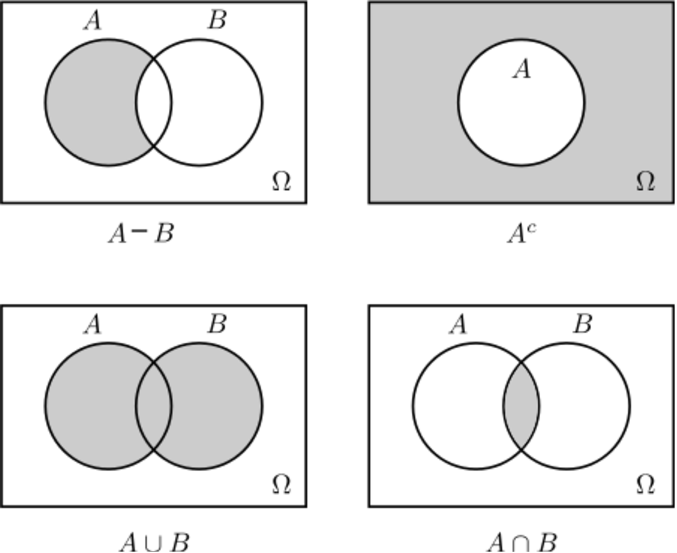
\includegraphics[angle=0, scale=0.72]{fig1-1.pdf}
\caption{\label{fig1} Operações básicas entre conjuntos.}
\end{center}
\end{figure} 
\end{frame}
%=====================================================================

%=====================================================================
\begin{frame}
 \begin{block}{Outras operações entre conjuntos}
 \begin{itemize}
   \item  $A \cap A = A.$
   \item $A \cup A = A.$
   \item $A \cap \emptyset = \emptyset.$
   \item $A \cup \emptyset = A.$ Elemento neutro da união.
   \item $A \cap \Omega= A.$ Elemento neutro da interseção.
   \item $A \cup \Omega = \Omega.$
   \item $A \cap B = B \cap A.$ Propriedade comutativa da interseção.
   \item $A \cup B = B \cup A.$ Propriedade comutativa da união.
   \item $\left(A^\complement\right)^\complement = A.$ Propriedade de involução.
   \item $(A \cap B) \cap C = A \cap (B \cap C).$ Propriedade associativa da interseção.
   \item $(A \cup B) \cup C = A \cup (B \cup C).$ Propriedade associativa da união.
   \item $A \cap (B \cup C) = (A \cap B) \cup (A \cap C).$ Propriedade distributiva da interseção.
   \item $A^\complement \cup B^\complement = (A \cap B)^\complement.$ Lei de De Morgan
   \item $A^\complement \cap B^\complement = (A \cup B)^\complement.$ Lei de De Morgan
   \item $A \cup (B \cap C) = (A \cup B) \cap (A \cup C).$ Propriedade distributiva da união
  \end{itemize}  
 \end{block}

\end{frame}
%=====================================================================

%=====================================================================
\begin{frame}
 
\frametitle{Leis de De Morgan para sequências.} 

Sejam $A_1, A_2, \ldots$ uma sequência de eventos (família de conjuntos) de $\Omega.$ 

\begin{enumerate}
\item $\cup_{i=1}^\infty A_i$ é o evento que ocorre quando pelo menos um dos eventos $A_i,$ $i=1,2,\ldots$ ocorre. 

\item $\cap_{i=1}^\infty A_i$ é o evento que ocorre quando todos os eventos $A_i,$ $i=1,2,\ldots$ ocorrem.

 \item $$\displaystyle{\left(\bigcup_{i=1}^\infty A_i\right)^\complement = \bigcap_{i=1}^\infty A_i^\complement}$$ Esta propriedade estabelece que o evento de que nenhum dos $A_i$'s aconteçam é igual ao complementar do evento de que pelo menos um dos $A_i$'s aconteça.
\item $$\left(\bigcap_{i=1}^\infty A_i\right)^\complement=\bigcup_{i=1}^\infty A_i^\complement$$ A propriedade expressa que o complementar do evento de que todos os $A_i$'s aconteçam é exatamente o evento de que pelo menos um deles não aconteça.
\end{enumerate}
\begin{exer}
	Verificar a validade das anteriores igualdades.
\end{exer}	
	
\end{frame}
%=====================================================================

%=====================================================================
\begin{frame}
% \frametitle{Função}
\begin{defi}[Função]
 Sejam $A$ e $B$ dois conjuntos. Se a cada elemento de um conjunto $A$ esta associado exatamente um único elemento do conjunto $B,$ então se diz que tal correspondência é uma função de $A$ em $B$ a qual é denotada por $f$ e se escreve como
$$
f: A \rightarrow B.
$$ O conjunto $A$ se chama o domínio da função e o conjunto $B$ é o  codomínio ou contradomínio de $f.$ 
\end{defi}
\begin{enumerate}
\item Se $a\in A,$ então o elemento de $B$ que corresponde a este $a,$ se chama a {\it imagem} de $a$ e é denotada por $f(a).$ Se $f$ é uma função de $A$ em $B$ e $b\in B$  então se define a {\it imagem recíproca} de $B$ como o conjunto de todos os elementos do conjunto $A$ que tem a $b$ como a sua imagem, isto quer dizer:
$$
f^{-1}(b):= \{ a\in A : f(a) = b \}.
$$
\item Se $C$ é um subconjunto de $B,$ então o conjunto de elementos de $A$ cujas imagens são elementos de $C,$ é chamado de {\it imagem recíproca de $C$ por $f$}  e a denotamos por  $f^{-1}(C).$ Isto é:
$$
f^{-1}(C) := \{ a\in A : f(a) \in C \}.
$$  
\item Se $D$ é um subconjunto de $A,$ então um subconjunto de $B$ cujos elementos são as imagens dos elementos de $D$ por meio da função $f$ se chama de {\it imagem direta} de $D$ e é denotada por $f(D),$ em que 
$$
f(D):=\{ b\in B :  b = f(a) \ \text{para algum} \ a\in D\} =  \{ f(a): a \in D \}.
$$
\end{enumerate}
\end{frame}
%=====================================================================



%=====================================================================
\begin{frame}{Cardinalidade}
\begin{enumerate}
	\item  Um subconjunto importante dos números  naturais é o conjunto de índices  $I_n = \{ p \in \mathbb{N},1 \le p \le n \}$  para algum  $n \in \mathbb {N} .$
	
	%  \item Um conjunto $A$ é finito se: i) ele é vazio. (Neste caso o conjunto não têm elementos) ii)
	% quando existe uma bijeção entre  $I_n$  e  $A$ . (Neste caso o conjunto têm $n$ elementos)
	% escreve-se  $f_{bij}:I_n \mapsto A$.
	% \end{enumerate}
	% Daqui observamos que:
	% \begin{itemize}
	\item Logo, todo conjunto  $I_n$  é finito.
	\item Seja $A$ um conjunto não vazio. Se existe $n \in \mathbb{N}$  e uma função injetiva  $g : A \mapsto I_n $ diremos que $A$ é finito, caso contrário,$A$ é infinito.
	\item O menor número $n$ que verifica esta propriedade é dito número de elementos de $A$. Escrevemos  $|A| = n$ . Diremos também que o conjunto vazio é finito e que seu número de elementos é 0.
	
	
	\item Uma função de bijeção entre dois conjuntos finitos ocorre somente quando eles possuem a mesma quantidade de elementos, aí dizemos que eles possuem a mesma cardinalidade. (De forma geral, se existe uma bijeção entre dois conjuntos, eles possuem a mesma cardinalidade, podendo eles serem infinitos).
	% \item Numa bijeção, se um conjunto é finito, o outro também o é ou se um não for finito o outro também não é.
	
\end{enumerate}

\begin{exem}
	Caso exista uma bijeção entre $A$ e  $I_5 = \{\omega_1, \omega_2, \omega_3, \omega_4, \omega_5 \} $, então $A$ possui 5 elementos. Resulta trivial demonstrar que esta função es bijetiva: $f: \{\omega_1, \omega_2, \omega_3, \omega_4, \omega_5 \}  \mapsto  {1,2,3,4,5}:$
	$$
	f(x) = \begin{cases} 
	1, & \text{se }x = \omega_1 \\ 
	2, & \text{se }x = \omega_2 \\ 
	3, & \text{se }x = \omega_3 \\
	4, & \text{se }x = \omega_4 \\
	5, & \text{se }x = \omega_5 
	\end{cases}
	$$
\end{exem}

\end{frame}
%=====================================================================

%=====================================================================
\begin{frame}
\begin{defi}[Produto cartesiano]
O {\it produto cartesiano} entre dois conjuntos $A$ e $B$ (denotado por $A \times B $) é um novo conjunto em que seus elementos são pares ordenados $(a,b),$ em que $a \in A$ e $b \in B.$ Simbolicamente, temos que 
$$
A \times B = \{ (a,b):  a \in A \ \text{e} \ b \in B \}.
$$ e em geral os conjuntos produto  $A \times B$ e $ B \times A $  são distintos uma vez que o par $(a,b)$ é distinto do par $(b,a).$ 
\end{defi}


\begin{exem}
O produto cartesiano $\mathbb{R}\times\mathbb{R}$ é o conjunto de todos os pares de números reais $(x,y)$ e o denotamos por $\mathbb{R}^2.$  De forma análoga são construídos os conjuntos $\mathbb{R}^3,$ $\mathbb{R}^4,....\mathbb{R}^k,...$ 
\end{exem}


Se a cardinalidade do conjunto $|A| = n$ e a cardinalidade do conjunto $|B|=m,$ então a cardinalidade de $|A \times B| = n m .$ Este resultado é conhecido como {\it princípio da multiplicação}. 
Em geral, a cardinalidade do produto cartesiano de $n$ conjuntos é
$$
|(A_1\times A_2 \times \cdots \times A_n)| = |A_1| \cdot |A_2|  \cdots \cdot | A_n|.
$$

\begin{exem} 
Seja $A=\{0,1\}.$  o conjunto  $  \underbrace{A\times A \times \cdots \times A}_{n}$ tem $2^n$ elementos.
\end{exem}
\end{frame}
\end{document}
%=====================================================================

\section{Experimento Aleatório}
\begin{frame}
\frametitle{\textbf{Experimento Aleatório}}
\baselineskip=13pt
\begin{block}{}
	
	Um {\em experimento} é qualquer processo de observação.
	
	\begin{itemize}
		\item Incerteza ou chance. Implica em falta de capacidade para
		de predizer seu comportamento em futuras realizações.
		
		\item Razões.
		
		\begin{itemize}
			\item não sabemos todas as causas envolvidas;
			
			\item não temos dados
			suficientes sobre as condições iniciais do experimento;
			
			\item as causas
			podem ser tão complexas que o cálculo do seu efeito combinado não é
			possível;
			
			\item existe alguma aleatoriedade fundamental no
			experimento, por exemplo, mecânica quântica;
		\end{itemize}
	\end{itemize}
\end{block}

\begin{block}{}
	
	Os seguintes
	traços caracterizam um experimento aleatório:
	
	\begin{enumerate}
		\item[(a)] Se for possível repetir as mesmas condições do
		experimento, os resultados do experimento em diferentes realizações
		podem ser diferentes.
		
		\item[(b)] Pode-se descrever o conjunto de
		todos os possíveis resultados do experimento.
		
		\item[(c)] quando o experimento for repetido um grande número de
		vezes, uma configuração definida ou regularidade surgirá. É esta
		regularidade que torna possível construir um modelo probabilístico.
	\end{enumerate}
	
\end{block}
\end{frame}


\begin{frame}
\frametitle{\textbf{Caracterização}}
\baselineskip=13pt
\begin{block}{}

Os resultados de um experimento aleatório são caracterizados pelos
seguintes componentes:

\begin{enumerate}
\item o conjunto de resultados possíveis $\Omega.$ 
\item a coleção de conjuntos de resultados de interesse $\A$;
\item um valor numérico $P$ da verosimilhança ou probabilidade de
ocorrência de cada um dos conjuntos de resultados de interesse.
\end{enumerate}

\end{block}
\end{frame}

%
\begin{frame}
\frametitle{\textbf{Espaço Amostral}}
\baselineskip=13pt
\begin{block}{}


O conjunto de possíveis resultados de um experimento aleatório é
chamado de {\em espaço amostral}  (SS = Sample Space). Existem quatro pontos que são
desejáveis da especificação de um espaço amostral:

\begin{enumerate}
\item[SS1.] listar os possíveis resultados do experimento;

\item[SS2.] fazê-lo sem duplicação;

\item[SS3.] fazê-lo em um nível de detalhamento suficiente para os
interesses desejados;

\item[SS4.] especificar essa lista completamente em um sentido
prático, embora usualmente não completa no que se refere a todos os
resultados logicamente ou fisicamente possíveis.
\end{enumerate}

(Este conjunto não necessariamente é único e sua
determinação depende do interesse do observador ou pessoa que realiza o
experimento aleatório).

\end{block}
		Espaços amostrais podem ser enumeráveis ou não enumeráveis;
se os elementos do espaço amostral podem ser colocados em uma correspondência 1-1 com um subconjunto
dos inteiros, o espaço amostral é enumerável.
\end{frame}
%
%
%\begin{frame}
%\frametitle{\textbf{Espaço Amostral}}
%\baselineskip=13pt
%
%\end{frame}



%=====================================================================
\begin{frame}
%\begin{block}{}
%	
%	

%	
%\end{block}
\begin{exem}
	Por exemplo, em uma única jogada de uma moeda poderíamos ter:
	\begin{itemize}
		\item $\Omega_1=\{cara,coroa\}$; $\Omega_2=\{cara,coroa,borda\}$; ou $\Omega_3=\{(x,y)\in \mathbb{R}^2\}$, onde $(x,y)$ são as coordenadas do centro da moeda após parar.
	\end{itemize}
	
	
\end{exem}

\begin{exem}
	Suponhamos que é selecionado ao acaso um estudante de uma sala de aula e é medida a sua altura. O resultado do experimento é a estatura, medida em metros.
	
	$$\Omega_1 = \{ x \in \mathbb{R}: x=1 + a_1 10^{-1} + a_2 10^{-2}, \ \text{com} \ a_1, a_2 \in \mathbb{N}_0 \ \text{e} \  a_1, a_2 \leq 10  \},$$  em que $\mathbb{N}_0$ é o conjunto dos números naturais incluindo o zero.  $\Omega_1$ indica que a estatura está medida em metros, com estatura mínima de um metro ($a_1=a_2=0$) e estatura máxima de dois metros e dez centímetros  ($a_1=a_2=10$). Este espaço amostral pode ser adequado para a população Brasileira sendo que um metro como estatura minima pode ser muito pequena. Em princípio, e de forma conceitual, a estatura é uma variável contínua. Assim, podemos propor como espaço amostral 
	$$\Omega_2 = [1 , \quad 2,1]  = \{ x \in \mathbb{R}: 1\leq x \leq 2,1 \},$$ 
	que reflete a possibilidade de mensurar a estatura com uma precisão absoluta,  com estatura mínima de exatamente um metro e máxima de dois metros e dez centímetros.
\end{exem}

\end{frame}

\begin{frame}
%\begin{block}{}
%	
%	

%	
%\end{block}

\begin{exem}
	 Outras possibilidades poderiam ser  
	$$\Omega_3 = (0 , \quad 100)  = \{ x \in \mathbb{R}: 0< x < 100 \},$$ e
	$$\Omega_4 = (0 , \quad \infty)  = \{ x > 0 \},$$ 
	Podemos pensar em $\Omega_3$ e $\Omega_4$ como exageros para o espaço amostral, não pelo fato da medição ser absoluta mas pela própria escala de variação dos valores. Contudo, estes dois espaços contêm os possíveis resultados de interesse. 
\end{exem}

\begin{exem}
	Observamos a posição de uma partícula que se move aleatoriamente sobre o eixo real. Aqui, $\Omega =\mathbb{R}.$
\end{exem}

\end{frame}
%=====================================================================




\begin{frame}
%\frametitle{\textbf{Eventos e Coleção de Eventos}}
%\baselineskip=13pt
%\begin{block}{}

\begin{block}{Eventos e Coleção de Eventos}
	\begin{itemize}
		 \item  o elemento $\omega \in \Omega$ é chamado de
		{\it evento elementar}, e todo subconjunto do espaço amostral  $A\subset\Omega$ é dito de  {\it evento}.
%		
%		\item Um {\em evento} é um subconjunto do espaço amostral.
%		
		\item Se ao
		realizarmos um experimento aleatório, o resultado pertence a um dado
		evento $A$, dizemos que $A$ {\em ocorreu}.
		
		\item Utilizaremos as operações Booleanas de conjuntos (complementar,
		união, intersecção, diferença) para expressar eventos combinados de
		interesse.
		
	\end{itemize}
	
\end{block}


\begin{block}{Eventos Disjuntos}
	
	%\begin{definition}
	Os eventos $A$ e $B$ s\~ao {\em disjuntos} ou {\em mutuamente excludentes}
	ou {\em mutuamente exclusivos} se n\~ao puderem ocorrer juntos.
%	, ou, em
%	linguagem de conjuntos, $A\cap B = \emptyset$.
	%\end{definition}
\end{block}

%\begin{block}{}
	
	\begin{exer}
	Sejam $A$, $B$, e $C$ eventos em um mesmo espaço amostral $\Omega$.
	Expresse os seguintes eventos em função de $A$,
	$B$, e $C$ e operações Booleanas de conjuntos (uniões, interseções, etc).
	\begin{description}
		\item[(a)] Pelo menos um deles ocorre:
		%\[ A\cup B\cup C.\]
		\item[(b)] Exatamente um deles ocorre:
		%\[ (A\cap B^c\cap C^c)\cup(A^c\cap B\cap C^c)\cup(A^c\cap B^c\cap C).\]
		\item[(c)] Apenas $A$ ocorre:
		%\[ (A\cap B^c\cap C^c).\]
		\item[(d)] Pelo menos dois ocorrem:
		%\[ (A\cap B\cap C^c)\cup(A\cap B^c\cap C)
		%\cup(A^c\cap B\cap C)\cup (A\cap B\cap C).\]
		\item[(e)] No m\'aximo dois deles ocorrem:
		%\[ (A\cap B\cap C)^c.\]
	%	\item[(f)] Nenhum deles ocorre:
		%\[ (A^c\cap B^c\cap C^c).\]
	%	\item[(f)] Ambos $A$ e $B$ ocorrem, mas $C$ não ocorre:
		%\[ (A\cap B\cap C^c).\]
	\end{description}
	\end{exer}
	
%\end{block}
\end{frame}
%
%\begin{frame}
%\frametitle{\textbf{Exemplos de Eventos}}
%\baselineskip=13pt
%\begin{block}{Eventos Disjuntos}
%
%%\begin{definition}
%Os eventos $A$ e $B$ s\~ao {\em disjuntos} ou {\em mutuamente excludentes}
%ou {\em mutuamente exclusivos} se n\~ao puderem ocorrer juntos, ou, em
%linguagem de conjuntos, $A\cap B = \emptyset$.
%%\end{definition}
%\end{block}
%
%\begin{block}{}
%
%%\begin{example}
%Sejam $A$, $B$, e $C$ eventos em um mesmo espaço amostral $\Omega$.
%Expresse os seguintes eventos em função de $A$,
%$B$, e $C$ e operações Booleanas de conjuntos.
%\begin{description}
%\item[(a)] Pelo menos um deles ocorre:
%%\[ A\cup B\cup C.\]
%\item[(b)] Exatamente um deles ocorre:
%%\[ (A\cap B^c\cap C^c)\cup(A^c\cap B\cap C^c)\cup(A^c\cap B^c\cap C).\]
%\item[(c)] Apenas $A$ ocorre:
%%\[ (A\cap B^c\cap C^c).\]
%\item[(d)] Pelo menos dois ocorrem:
%%\[ (A\cap B\cap C^c)\cup(A\cap B^c\cap C)
%%\cup(A^c\cap B\cap C)\cup (A\cap B\cap C).\]
%\item[(e)] No m\'aximo dois deles ocorrem:
%%\[ (A\cap B\cap C)^c.\]
%\item[(f)] Nenhum deles ocorre:
%%\[ (A^c\cap B^c\cap C^c).\]
%\item[(g)] Ambos $A$ e $B$ ocorrem, mas $C$ não ocorre:
%%\[ (A\cap B\cap C^c).\]
%\end{description}
%%\end{example}
%
%\end{block}
%\end{frame}

%
\begin{frame}
%%\frametitle{\textbf{Partição}}
%%\baselineskip=13pt
%\begin{block}{}
 \begin{defi}[Partição] Dado um espaço amostral $\Omega$, uma partição
$\Pi=\{A_{\alpha},\alpha\in\I\}$ de $\Omega$ é uma coleção de
eventos que satisfaz:
\begin{enumerate}
\item[P1.] Para todo $\alpha\neq\beta$, $A_{\alpha}\cap
A_{\beta}=\emptyset$;
%
\item[P2.] $\cup_{\alpha\in\I}A_{\alpha}=\Omega.$
\end{enumerate}
\end{defi}
%\end{block}
%
%\begin{block}{}

Portanto, cada elemento
$\omega\in\Omega$ pertence a um, e somente um, dos eventos
$A_{\alpha}$ de uma partição.

\begin{exem}
	A coleção de intervalos $\{(n,n+1]:n \in \mathbb{Z} \}$ é uma partição dos
números reais $\mathbb{R}$. 
\end{exem}

%\end{block}
\end{frame}
%
%
\begin{frame}
\frametitle{\textbf{Álgebra de Eventos}}
\baselineskip=13pt
\begin{block}{}


Por que não analisar todos os subconjuntos de um dado espaço amostral?
\begin{itemize}
\item o espaço amostral pode conter um grau de
detalhamento superior ao que estamos interessados no momento;

\item quereremos associar cada
evento $A$ com uma probabilidade numérica $P(A)$, porém nosso conhecimento sobre $P$ pode não
estender para todos os subconjuntos de $\Omega$;

\item Axiomas de Kolmogorov podem implicar que não exista $P$ definida em
todos os subconjuntos de $\Omega$ (não enumerável).
\end{itemize}

Estaremos interessados em uma coleção especial $\A$ de subconjuntos do espaço amostral
chamada de uma {\em álgebra de eventos}.

\end{block}
\end{frame}
%
\begin{frame}
\frametitle{\textbf{Álgebra de Eventos}}
%\baselineskip=13pt
%\begin{block}{}

\begin{definition}
Uma álgebra de eventos $\A$ é uma coleção de subconjuntos do espaço
amostral $\Omega$ que satisfaz:

\begin{enumerate}
\item não é vazia;

\item fechada com respeito a complementos (se $A\in\A$, então
$A^c\in\A$);

\item fechada com respeito a uniões finitas (se $A,B\in\A$, então $A\union
B\in\A$).
\end{enumerate}
\end{definition}

{\bf Observação:} Pelas Leis de De Morgan, vemos que $\A$ é fechada com respeito a
intersecções finitas também.

%\end{block}
\end{frame}
%
\begin{frame}
\frametitle{\textbf{Exemplos de Álgebra de Eventos}}
%\baselineskip=13pt
%\begin{block}{}


%\begin{example}
\begin{enumerate}
\item A menor álgebra de eventos é $\A=\{\emptyset,\Omega\}$;
\item A maior álgebra de eventos é o conjunto das partes de
$\Omega$;
\item Um exemplo intermediário, temos:
$$\Omega=\{1,2,3\}\mbox{, }\A=\{\Omega,\emptyset,\{1\},\{2,3\}\}.$$
\item A álgebra de eventos finitos e co-finitos (conjuntos cujo complemento é finito). Seja $\Omega=\IR$ e
$$\A=\{A\subseteq \IR:A\mbox{ é finito}\}\cup\{A\subseteq \IR:A^c\mbox{ é finito}\},$$
ou seja, $\A$ consiste dos subconjuntos de $\IR$ que ou são finitos ou têm complementos finitos.
$\A$ é uma álgebra de eventos.
\end{enumerate}
%\end{example}
%
%\end{block}
\end{frame}
%
\begin{frame}
\frametitle{Propriedades de Álgebra de Eventos}

\vspace{-0.1cm}
\begin{lema} Se $\A$ é uma álgebra, então $\Omega\in\A$ \end{lema}

\begin{proof} Como $\A$ é não vazia, seja $A$ um elemento qualquer seu. Pela
segunda propriedade de álgebras, temos que $A^c\in\A$, e pela
terceira propriedade temos que $\Omega=A\union A^c\in\A$. \end{proof}

\begin{teo} \label{interalgebra}Sejam $\A_1$ e $\A_2$ álgebras de subconjuntos de $\Omega$ e
seja $\A=\A_1\inter \A_2$ a coleção de subconjuntos comuns as duas
álgebras. Então, $\A$ é uma álgebra. \end{teo}

\begin{proof} Como $\A_1$ e $\A_2$ são álgebras, ambos contém $\Omega$.
Então, $\Omega\in\A$. Se $A\in\A$, então $A$ está em ambos $\A_1$ e
$\A_2$. Logo, $A^c$ está em ambos $\A_1$ e $\A_2$, e portanto na sua
intersecção $\A$. Se $A,B\in\A$, então eles estão em ambos $\A_1$ e
$\A_2$. Consequentemente, $A\union B$ está em ambos $\A_1$ e $\A_2$
e, portanto, em $\A$. Como $\A$ satisfaz as três condições da
definição de álgebra de eventos, $\A$ é uma álgebra de eventos.
\end{proof}

\end{frame}
%
\begin{frame}
%\frametitle{\textbf{Propriedades de Álgebra de Eventos}}
%\baselineskip=13pt
%\begin{block}{}


É fácil ver que a prova do
%Teorema~\ref{interalgebra}
teorema anterior pode ser estendida para o caso
de uma intersecção de um número arbitrário de álgebras. O seguinte corolário usa este fato
para provar que sempre existe uma menor álgebra contendo uma família qualquer de eventos.

\begin{corol} Existe uma menor (no sentido de inclusão) álgebra contendo
qualquer família dada de subconjuntos de $\Omega$. \end{corol}
\begin{proof}
Seja $\C$ uma coleção qualquer de subconjuntos de $\Omega$, defina $\A(\C)$ como sendo o conjunto que é igual a intercessão de todas as álgebras de eventos que contém $\C$, isto é:
$$\A(\C)=\bigcap_{\A\supseteq\C:\A\mbox{ é uma álgebra de eventos}}\A.$$
Pelo
%Teorema~\ref{interalgebra}
teorema anterior, $\A(\C)$ é uma álgebra de eventos, e consequentemente é a menor álgebra de eventos contendo $\C$. $\A(\C)$ é conhecida como a {\em álgebra de eventos gerada por $\C$}.
\end{proof}
%
%\end{block}
\end{frame}
%
\begin{frame}
%\frametitle{\textbf{Propriedades de Álgebra de Eventos}}
%\baselineskip=13pt
%\begin{block}{}

\begin{teo} Se $\A$ é uma álgebra de eventos, então
$$A_i\in\A,i=1,2,\ldots,n\Rightarrow \union_{i=1}^{n}A_i \in \A$$
\end{teo}

\begin{proof} Para $n=1$, o resultado é óbvio. Para $n=2$, o resultado segue
diretamente da terceira propriedade na definição de álgebra de
eventos. Vamos agora provar o passo indutivo, suponha que
$$A_i\in\A,i=1,2,\ldots,k\Rightarrow \union_{i=1}^{k}A_i \in \A.$$
Vamos agora provar que o caso $n=k+1$ é verdadeiro. Suponha que
$A_i,i=1,2,\ldots,k+1\in\A$, então como
$$\union_{i=1}^{k+1}A_i=(\union_{i=1}^{k}A_i)\union A_{k+1},$$
temos que utilizando o caso $n=k$, $\union_{i=1}^{k}A_i\in\A$. Como $\union_{i=1}^{k}A_i\in\A$ e $A_{k+1}\in \A$, temos que utilizando o caso $n=2$, $(\union_{i=1}^{k}A_i)\union A_{k+1}\in \A$.
\end{proof}

%\end{block}
\end{frame}

\begin{frame}
\frametitle{Construindo uma Álgebra de Eventos}


\begin{nota} Uma maneira de construir uma álgebra de eventos, é primeiro
particionar $\Omega$ em um número finito subconjuntos e depois considerar álgebra que consiste
dos eventos que são uniões finitas dos subconjuntos da partição. \end{nota}

\begin{exem}
Por exemplo, $\Omega=\{a,b,c,d\}$. Considere a partição,
$\{\{a,c\},\{b,d\}\}$, então considere a coleção de eventos que consiste de uniões finitas dos eventos desta
partição: $\A=\{\emptyset, \Omega, \{a,c\},\{b,d\}\}$. É fácil ver
que $\A$ é uma álgebra de eventos.
\end{exem}

\end{frame}
%
\begin{frame}
%\frametitle{\textbf{Construindo uma Álgebra de Eventos}}
%\baselineskip=13pt
%\begin{block}{}

\begin{defi}
Dada uma coleção finita eventos $\C=\{A_1,A_2,\ldots,A_n\}$, define-se um {\bf  átomo} de $\C$ como sendo qualquer evento
$B$ da seguinte forma: $B=B_1\cap B_2\cap\ldots\cap B_n$, onde $B_i=A_i$ ou $B_i=A_i^c$ para $i=1,2,\ldots,n$.
\end{defi}
Note que existem no máximo $2^{|\C|}$ átomos diferentes e que eles formam uma partição de $\Omega$ (verifique!). Quando $\C$ for uma coleção finita de eventos, um evento pertencerá a $\A(\C)$, se e somente se,
for igual a uma união finita de átomos de $\C$. Note que $\A(\C)$ terá no máximo $2^{2^{|\C|}}$ elementos (verifique!).

\begin{exem}
Se $\Omega=\{a,b,c,d,e,f\}$, encontre a álgebra gerada por $\C=\{\{a,b,d\},\{b,d,f\}\}$.

Note que Os átomos de $\C$ são
$\{\{a\},\{f\},\{c,e\},\{b,d\}\}$. Logo,
\begin{eqnarray}
& & \A(\C)=\{\emptyset,\Omega,\{a\},\{f\},\{c,e\},\{b,d\},\{a,f\},\{a,c,e\},\nonumber \\
& & \{a,b,d\}, \{c,e,f\},\{b,d,f\},\{b,c,d,e\},\{a,f,c,e\},\nonumber \\
& & \{a,f,b,d\},\{a,b,c,d,e\},\{b,c,e,d,f\}\}.\nonumber
\end{eqnarray}
\end{exem}
%
%\end{block}
\end{frame}
%
%
%

\end{document}

%=====================================================================
 \begin{frame}
 \begin{defi}[Função Indicadora]
 Seja $\Omega$ o espaço amostral e ${\cal F}$ uma coleção de subconjuntos de $\Omega.$ A função indicadora de um conjunto $A \in {\cal F} $ é denotada por $\mathbf{1}_A(x)$ e é definida por 
 $$
\mathbf{1}_A(x) = 
\begin{cases}
1 &\text{se}\ x \in A, \\
0 &\text{se}\ x \notin A. 
\end{cases} = 
\begin{cases}
1 &\text{se}\ x \in A, \\
0 &\text{se}\ x \in A^c = X - A. 
\end{cases}
 $$
 \end{defi}
 
Sejam $A$ e $B$ subconjuntos de $\Omega$ então:
 \begin{enumerate}
\item $\mathbf{1}_{A\cap B} = \min\{\mathbf{1}_A,\mathbf{1}_B\} = \mathbf{1}_A \cdot\mathbf{1}_B,\,$ (interseção de conjuntos)
\item $\mathbf{1}_{A\cup B} = \max\{{\mathbf{1}_A,\mathbf{1}_B}\} = \mathbf{1}_A + \mathbf{1}_B - \mathbf{1}_A \cdot\mathbf{1}_B,$ (união de conjuntos)
\item $\mathbf{1}_{A\Delta B} = \max\{{\mathbf{1}_A,\mathbf{1}_B}\} = \mathbf{1}_A + \mathbf{1}_B - 2 \cdot \mathbf{1}_A \cdot\mathbf{1}_B, $(diferença simétrica de conjuntos)
\item $\mathbf{1}_{A^\complement} = 1-\mathbf{1}_A.$ (complemento de um conjunto)
 \item Suponhamos que $A_1, \ldots, A_n$ é uma coleção de subconjuntos de $ {\cal F}  $ e seja $I_n = \{1,2,3,...,n\}$ como o conjunto de índices, então
 $$ \prod_{k \in I_n} ( 1 - \mathbf{1}_{A_k}(\omega)),$$  para todo $\omega \in \Omega. $
 é claramente um produto de 0's e 1's. Este produto vale 1 precisamente para os $\omega \in \Omega$ que não pertencem a nenhum dos conjuntos $A_k$ e 0 em caso contrário. Isto é,
  $$\prod_{k \in I_n} ( 1 - \mathbf{1}_{A_k}) = \mathbf{1}_{\Omega - \bigcup_{k} A_k} = 1 - \mathbf{1}_{\bigcup_{k} A_k}.$$
\end{enumerate}
% 
% 
% 
 \end{frame}
%=====================================================================

%=====================================================================
\begin{frame}
\begin{exem}
$$f(x)= \begin{cases}
0 \ , & x <-1\\
1+x \ , & -1 \leq x < 0\\
1-x \ , & 0 \leq x < 1\\
0 \ , & x \geq 1
\end{cases} $$
Note que $f(x)$ pode ser escrita como 
$$
f(x)=(1+x)\mathbf{1}_{[-1,0)}(x)+(1-x)\mathbf{1}_{[0,1)}(x),
$$
ou de forma mais compacta como
$$f(x)=(1-\vert x\vert)\mathbf{1}_{[-1,1]}(x) $$
\end{exem}
\end{frame}
%=====================================================================
%=====================================================================
\begin{frame}{Elementos de probabilidade}
\begin{enumerate}
 \item A teoria da probabilidade é uma parte da matemática que nasceu no esforço de modelar {\it jogos de azar}
 \item A teoria da probabilidade se ocupa do estudo dos fenômenos ou experimentos aleatórios (experimentos nos quais é impossível prever com antecipação o seu resultado ao serem repetidos inúmeras vezes sob as mesmas condições).
 
\end{enumerate}
\begin{block}{Algumas definições}
\begin{enumerate}
 \item O conjunto $\Omega$ (omega) de todos os possíveis resultados do experimento é chamado de {\it espaço  amostral}. Este conjunto não necessariamente é único e sua determinação depende do interesse do observador ou pessoa que realiza o experimento aleatório.
 \item O conjunto $\Omega$ (omega) de todos os possíveis resultados do experimento é chamado de {\it espaço  amostral}.  Este conjunto não necessariamente é único e sua determinação depende do interesse do observador ou pessoa que realiza o experimento aleatório.
 \item  o elemento $\omega \in \Omega$ é chamado de
{\it evento elementar}, e todo subconjunto do espaço amostral  $A\subset\Omega$ é dito de  {\it evento}.
\item  Um evento $B$ é dito que aconteceu, se e somente se, o resultado observado $\omega$ do experimento é um elemento de $B.$
 \end{enumerate}
\end{block}
\end{frame}
%=====================================================================



%=====================================================================
\begin{frame}
Em um experimento aleatório nem  todos os subconjuntos do espaço amostral são eventos. Para
tanto, exigimos que a classe de subconjuntos para os quais estará definida a
``chance'' de ocorrência seja uma {$\sigma$-álgebra}.

\begin{defi}[{$\sigma$-álgebra}]
Seja $\Omega\neq \emptyset.$  Uma classe (família) de eventos ${\cal F}$  é uma {$\sigma$-álgebra} sobre $\Omega,$  se e somente se, são satisfeitas as 
as seguintes propriedades: 
\begin{enumerate}

\item Se $A\in{\cal F},$ então $A^c\in{\cal
F},$  
\item $\Omega \in {\cal F},$ 
\item  Se $A_1, A_2, \ldots, \in {\cal F},$ 
então \ $\bigcup_{i=1}^\infty A_i \in {\cal F}.$ 
\end{enumerate}
\end{defi}

Da definição de  $\sigma$-álgebra é claro que $\Omega$ e $\emptyset$ pertencem a qualquer $\sigma$-álgebra definida sobre $\Omega.$
No caso dos eventos,  $\Omega$ é chamado de {\it evento certo} e $\emptyset$ é chamado de {\it evento impossível}.

\begin{exem}
\begin{enumerate}
\item  Se $\Omega\neq \emptyset,$ então $\{\Omega, \emptyset \}$ é a menor
$\sigma$-álgebra que pode ser definida sobre $\Omega.$  ($\sigma$-álgebra trivial). 

\item Se $\Omega  = \{ 1, 2, 3 \},$ então ${\cal F} = \{  \emptyset, \{ 1 \}, \{ 2, 3 \}, \Omega \} $ é uma $\sigma$-álgebra sobre $\Omega.$ 
% No entanto, a família 
% ${\cal G} = \{  \emptyset, \{ 1 \}, \{ 2 \},  \{ 3\}, \Omega \} $ não é uma $\sigma$-álgebra. 

\item  Se $\Omega\neq \emptyset,$ então $ \mathcal{P}(\Omega )$ a coleção de todos os subconjuntos de $\Omega$ (partes de $\Omega$) é uma $\sigma$-álgebra ($\sigma$-álgebra total). Em particular, seja $\Omega\neq \emptyset,$ finito e enumerável (caso discreto), e seja ${\cal F}$ uma 
$\sigma$-álgebra que contém todos todos os conjuntos da forma $\{ \omega \}$ com $\omega \in \Omega.$ Então, 
${\cal F} = \mathcal{P}(\Omega )$ é uma $\sigma$-álgebra.



 \end{enumerate} 
\end{exem} 
 

\end{frame}
%=====================================================================

%=====================================================================
\begin{frame}
\begin{exem}
\begin{enumerate}

\item ($\sigma$-álgebra gerada). Seja $\Omega\neq \emptyset$ e ${\cal L}$ uma coleção de subconjuntos de $\Omega.$ Seja $${\cal  M}=\{{\cal F}: {\cal F} \ \text{é uma $\sigma$-álgebra que contem a} \quad {\cal L}  \},$$ então, 
$$\sigma({\cal L}) = \bigcap_{{\cal F} \in {\cal M}}{\cal F}$$ é a menor $\sigma$-álgebra sobre $\Omega$ que contem a ${\cal L}.$ Esta $\sigma$-álgebra é a $\sigma$-álgebra gerada por ${\cal L}.$

\item  Se $\Omega =\mathbb{R}$ é o conjunto dos números reais. Seja ${\cal U}$ a
coleção formada por uniões disjuntas de intervalos da forma $(a,b]$, então
${\cal U}$  é uma $\sigma$-álgebra. Em particular, a menor $\sigma$-álgebra
sobre $\mathbb{R}$ que contém todos os intervalos da forma $(-\infty,a]$ com $a
\in \mathbb{R}$ se chama $\sigma$-álgebra de Borel e a denotamos por ${\cal
B}.$ Sendo $\mathbb{Q}$ o conjunto dos números racionais, temos que, os conjuntos 
$(a, \infty)=\mathbb{R}-(-\infty,a],$ 
$(a,b]=(-\infty, b]\cap (a, \infty),$  
$(-\infty,a)=\bigcup_{n=1}^\infty(-\infty,a- 1/n],$ $[a,\infty) = \mathbb{R}-(-\infty, a),$
$(a,b) = (-\infty, b)\cup (a, \infty),$ $[a,b] = \mathbb{R}-((-\infty, a)\cup
(b, \infty)),$  $\{a\}=[a,a],$ $\mathbb{N}=\bigcup_{n=0}^\infty\{n\},$
$\mathbb{Q}=\bigcup_{r \in \mathbb{Q}}\{r\}$ e
$\mathbb{Q}^c=\mathbb{R}-\mathbb{Q}$  são conjuntos da $\sigma$-álgebra de Borel
em $\mathbb{R}.$

 \end{enumerate} 

\end{exem} 
 \begin{nota}
  Nem todos os subconjuntos de $\mathbb{R}$ pertencem à $\sigma$-álgebra de Borel. Exemplo o conjunto de {\it Cantor.} Maiores detalhes ver [Gary L. Wise and Eric B. Hall, Counterexamples in Probability and Real Analysis. Oxford University Press, New York 1993]
 \end{nota}

 
\end{frame}
%=====================================================================

%=====================================================================
\begin{frame}
\begin{defi}[Espaço mensurável]
Se ${\cal F}$ é uma $\sigma$-álgebra
não vazia de subconjuntos de $\Omega,$  a dupla $(\Omega, {\cal F})$ é chamada
de {\it espaço mensurável} e os subconjuntos de $\Omega$ são chamados de
{\it conjuntos mensuráveis}. 
\end{defi}



\begin{defi}[Medida] Seja  $(\Omega, {\cal F})$  um espaço mensurável. Uma {\bf medida} sobre  $(\Omega, {\cal F})$  é uma função $\mu$ 
definida sobre ${\cal F}$ que assume valores em $\mathbb{R} \cup \{\infty\}$ tais que:
\begin{enumerate}
\item  $\mu (A) \geq 0$ para todo $A \in {\cal F},$

\item  $\mu(\emptyset)$ = 0,
\item  ($\sigma$-aditividade)   Para toda sequência $E_{1},E_{2},\ldots$ de conjuntos disjuntos dois a dois de ${\cal F} $ $$\mu \left( \bigcup _{i=1}^{\infty }E_{i}\right) =\overset{\infty }{%
\underset{i=1}{\sum }}\mu \left( E_{i}\right) .$$ 
\end{enumerate}
\end{defi}

Intuitivamente, a medida de um conjunto pode ser interpretada como o seu tamanho. Neste sentido, uma medida é uma generalização dos conceitos de comprimento, área e volume.

\begin{nota}
Para cada $A\in \frak{F}$,  o número $\mu \left( A\right) $ se chama a {\it medida de $A$} e a tripla $\left( \Omega ,\frak{F,\mu }\right) $ recebe o nome de
{\it espaço de medida.} Além disso, dizemos que a medida $\mu $ é {\it finita} se $\mu \left( \Omega \right) <\infty .$
\end{nota}
 
\end{frame}
%=====================================================================

%=====================================================================
\begin{frame}
\begin{exem}

\begin{enumerate}
\item  Seja $\Omega \neq \emptyset $ e seja ${\cal F}$ $\ $ uma $\sigma$-álgebra em $\Omega $, se fixamos um ponto $\omega\in \Omega ,$ definimos para cada $E\in {\cal F}$ : 
\begin{equation*}
\mu (E)=\delta_{\omega}(E)=\left\{ 
\begin{array}{c}
0,\text{ se} \ \omega\notin E \\ 
1,\text{ se}\ \omega\in E
\end{array}
\right.
\end{equation*} então $\mu $ é uma medida finita chamada de \emph{ medida de Dirac.}

\item  Seja $\Omega =\mathbb{N}$ e ${\cal F}=\mathcal{P}(\mathbb{N})$, para
cada $E\subseteq \mathbb{N}$ definimos uma medida $\mu (E)$ como o
n\'{u}mero de elementos de $E,$ se $E$  é finito e como $+\infty $ se $E$ é
infinito. Como podemos ver esta medida não é finita. Esta medida é chamada de \emph{medida de contagem} em  $\mathbb{N}.$

\item Seja $\Omega =\mathbb{R}$ e ${\cal F} = {\cal B}$ a $\sigma$-álgebra de Borel. Definimos $\mu((a, b]) = b - a$, (comprimento do
intervalo $(a,b]$) em que $a, b \in  \mathbb{R}.$ Esta medida é chamada de {\it medida de Lebesgue} na reta real.

\end{enumerate}
\end{exem}

\end{frame}
%=====================================================================

%=====================================================================
\begin{frame}


\begin{defi}[Frequência relativa] 
Para cada evento $A \in {\cal A}$ o número $f_r(A)={n(A)}/{n}$ se chama frequência
relativa de $A,$ onde $n(A)$ indica o número de vezes que ocorre o evento $A.$
\end{defi}

\begin{exem}
\begin{enumerate}
\item Uma moeda foi lançada 1000 vezes e forneceu 502 caras. Então a frequência relativa de ``caras'' é: 
$f_r(A) = 502 / 1000 = 0,502 = 50.2\%.$
\item Um dado foi lançado 1000 vezes e a face 6 apareceu 20 vezes. Então a frequência relativa do evento $A = \{ \text{face} \ 6 \}$ é: 
$f_r(A)  = 20 / 1000 = 0,02 = 2\% .$
\end{enumerate}
\end{exem}

 \begin{block}{Propriedades da frequência relativa:} 
Sejam $A$ e $B$ dois eventos do espaço amostral associado $\Omega$. Sejam $f_r(A)$   e $f_r(B)$ as frequências relativas de $A$ e $B$ respectivamente. Então, 
\begin{enumerate}
\item $ 0 \leq f_r(A) \leq 1$, isto é, a frequência relativa do evento $A$ é um número que varia entre 0 e 1. 
\item  $f_r(A)=1,$  se e somente se, $A$ ocorre em todas as $n$ repetições do experimento aleatório. 
\item  $f_r(A)=0$, se e somente se, $A$ nunca ocorre nas $n$ repetições do experimento aleatório. 
\item  $f_r(A \cup B)= f_r(A) + f_r(B),$ se $A$ e $B$ forem eventos mutuamente excludentes. 
\end{enumerate}
 \end{block}
 


\end{frame}
%=====================================================================

%=====================================================================
\begin{frame}

 \begin{defi}
Seja $A$ um evento de um espaço amostral $\Omega$. Suponhamos que o experimento  é repetido $n$ vezes e seja $f_r(A)$ a frequência relativa do evento. Então, a probabilidade de $A$ é definida por 
$$
P(A) = \lim_{n \rightarrow \infty} f_r(A) = \lim_{n \rightarrow \infty} \frac{n(A)}{n}.
$$
\end{defi}

Note que a frequência relativa do evento $A$ é uma aproximação da probabilidade de $A$.  Em geral, para um valor de $n$, razoavelmente grande, a $f_r(A)$ é uma boa aproximação de $P(A).$

 \begin{nota}[Crítica à definição frequentista da probabilidade]
A definição frequentista da probabilidade, embora útil na prática, apresenta dificuldades matemáticas, pois o limite pode não existir.
\end{nota}

\end{frame}
%=====================================================================

%=====================================================================
\begin{frame}{Definição de probabilidade}
O objetivo da probabilidade é atribuir a cada evento $A$ um número real
não-negativo que indique a ``chance'' que $A$ tem de acontecer. Suponhamos que
realizamos um experimento aleatório $n$ vezes e que as condições em que é
realizado permanecem relativamente constantes.

\begin{defi}[Medida de Probabilidade (Kolmogorov - 1956)] 
Seja $(\Omega, {\cal F})$ um espaço mensurável, uma função $P$ definida sobre
${\cal F}$ a valores reais que satisfaz (os axiomas):
\begin{enumerate}
 \item[A.1]$P(A)\geq 0,$ para todo $ A\in {\cal F},$
\item[A.2] $P(\Omega)=1,$ (medida finita).
\item[A.3] ($\sigma$-aditividade) Se $A_1, A_2, \ldots$ é uma sequência de eventos de
${\cal F}$  mutuamente excludentes, i.e., $A_i\cap A_j=\emptyset$ para todo
$i\neq j,$ então 
\begin{equation}
\displaystyle
\label{ax3}
P\left(\bigcup_{i=1}^\infty A_i\right)=\sum_{i=1}^\infty P(A_i)
\end{equation}
\end{enumerate}
se chama {\it medida de probabilidade} sobre $(\Omega, {\cal F})$  e a
tripla $(\Omega, {\cal F}, P)$ se chama {\it espaço de probabilidade}.
\end{defi}

Note que  uma vez que $P(\Omega)=1,$ o conjunto $\Omega$ é chamado de {\it evento certo} e $\emptyset$ é chamado de {\it evento impossível}.
\end{frame}
%=====================================================================

%=====================================================================
\begin{frame}
 \begin{exem}
 Seja $\Omega=\{ \clubsuit,  \heartsuit, \spadesuit \},$ ${\cal F}= \{ \emptyset, \Omega, \{ \clubsuit \}, \{  \heartsuit, \spadesuit \}    \}$ e $P$ a aplicação
definida sobre ${\cal F}$ da seguinte forma: 
\begin{equation}
\label{medp1}
P(A)=
\begin{cases}
 1, & \text{se} \quad \heartsuit \in A, \\
0, & \text{se} \quad \heartsuit \notin A \\
\end{cases}
\end{equation}
então, $P$ é uma medida de probabilidade sobre $(\Omega, {\cal F}).$
\end{exem}

\begin{exem}
 Seja $\Omega=\{ \clubsuit,  \heartsuit   \},$ ${\cal F}=\mathcal{P}(\Omega )$ e $P$ a aplicação
definida sobre ${\cal F}$ da seguinte forma: 
\begin{equation}
\label{medp2}
P(A)=
\begin{cases}
 0, & \text{se} \quad A =\emptyset, \\
2/5, & \text{se} \quad A =\{\heartsuit\}, \\
3/5, & \text{se} \quad A =\{\clubsuit\}, \\
1, & \text{se} \quad A =\{\clubsuit,  \heartsuit\}, \\
\end{cases}
\end{equation}
então, $P$ é uma medida de probabilidade.
\end{exem}

\begin{defi}[Espaço de probabilidade completo]
Seja $(\Omega, {\cal F}, P)$ um espaço de probabilidade. Qualquer evento $A$ tal
que $P(A)=0$ se chama evento nulo e o espaço $(\Omega, {\cal F}, P)$ se diz que é completo se
todos os subconjuntos de eventos nulos são eventos nulos.
\end{defi}

\end{frame}
%=====================================================================
% 
%=====================================================================
\begin{frame}{Propriedades da probabilidade}
Seja $(\Omega, {\cal F}, P)$ um espaço de probabilidade então $P$ satisfaz as seguintes propriedades:

\begin{enumerate}
\item[P.0] $P(\emptyset)=0.$ De fato, $1=P(\Omega)=P(\Omega \cup \emptyset \cup \emptyset\cup \emptyset\cup \emptyset \cdots )$ $=P(\Omega)+P(\emptyset)+P(\emptyset)+P(\emptyset)+\cdots,$  se e somente se,  $0 \leq P(\emptyset)\leq 1$ caso contrário contradiz [A.2].

\item[P.1] Seja $A$ um evento de ${\cal F}$  e $A^\complement$ o evento complementar, então $$P(A) = 1 - P\left(A^\complement\right).$$ 
De fato, sendo $ \Omega $ o espaço amostral, temos que $\Omega=A\cup A^\complement$ onde a união é disjunta, uma vez que $ A\cap A^\complement=\emptyset $. Utilizando [A.3]  segue que
$$P(\Omega)=P(A)+P\left(A^\complement\right)\Rightarrow P\left(A^\complement\right)=P(\Omega)-P(A)=1-P(A).$$ 


\item[P.2] A probabilidade de ocorrência de eventos associados a um experimento pode ser calculada através da regra da soma da probabilidade para a união de dois eventos. 
Sejam $A$ e $B$  dois eventos em  ${\cal F}$ a probabilidade da união destes dois eventos  é dada por $$ P(A\cup B) = P(A)+P(B)-P(A\cap B).$$ 
De fato, se $ A\cup B=A\cup (B- A) $ e $ A\cap(B - A)=\emptyset $, então $P(A\cup B)=P(A)+P(B - A).$ Agora para $ B=(B- A)\cup(A\cap B) $ com $ (B - A)\cap(A\cap B)=\emptyset $, então
$P(B)=P(B -s A)+P(A\cap B).$ Combinando estes dois resultados, temos que \[P(A\cup B)=P(A)+P(B)-P(A\cap B).\]
\end{enumerate}
 \end{frame}
%=====================================================================

%=====================================================================
\begin{frame}
\begin{enumerate}
\item[P.3]  Sejam $A$, $B$ e $C$ três eventos em ${\cal F}$, então 
$$
\begin{aligned}
P(A\cup B\cup C) & = P(A)+P(B)+P(C)-P(A\cap P) \\ &-B(A\cap C)-P(B\cap C)+P(A\cap B\cap C).
\end{aligned}
$$ 
De fato, temos que $A\cup B\cup C=(A\cup B)\cup C=(A\cup B)\cup (C - (A\cup B))$ por ser esta união disjunta. Então por [A.3], temos 
\begin{equation}
\label{eqp1}
P(A\cup B\cup C)=P(A\cup B)+P(C - (A\cup B)) 
\end{equation} 
e utilizando a equação \eqref{eqp1} temos 
$P(A\cup B\cup C)=P(A)+P(B)-P(A\cap B)+P(C - (A\cup B)).$ Mas, $$ C=(C - (A\cup B))\cup(C\cap(A\cup B)),$$ portanto \begin{equation}
\label{eqp2}
P(C - (A\cup B))=P(C)-P(C\cap(A\cup B)).
\end{equation}	
Além disso, temos que $ C\cap (A\cup B)=(C\cap A)\cup (C\cap(B -  A)) $, e esta união é disjunta. Logo,  
\begin{equation}
\label{eqp3}
P(C\cap (A\cup B))=P(A\cup C)+P(C\cap(B - A)).
\end{equation} 	
Finalmente, para $ C\cap B = (A\cap B\cap C)\cup (C\cap(B - A)) $, o que implica que 
\begin{equation}
\label{eqp4}
P(C\cap(B - A))=P(B\cap C) - P(A\cap B\cap C),
\end{equation} 		
já que a união é disjunta. Combinando as equações \eqref{eqp1}, \eqref{eqp2}, \eqref{eqp3} e \eqref{eqp4}, concluímos que 
\[
\begin{aligned}
P(A\cup B\cup C)&=P(A)+P(B)+P(C) - P(A\cap B) \\ & - P(A\cap C)  - P(B\cap C)  +P(A\cap B\cap C).
\end{aligned}
\]
\end{enumerate}
 \end{frame}
%=====================================================================

%=====================================================================
\begin{frame}
\begin{enumerate}
\item[P.4] Sejam  $A$ e $B$ eventos de ${\cal F}$ com $A  \subset  B$, então $P(A) \leq P(B).$ De fato, temos que se $ A\subset B $ então $ B = A\cup (B - A) $ e  $ \emptyset = A\cap (B - A) .$  Portanto, utilizando [A.3] segue que 
\[P(B)=P(A)+P(B- A).\] 	 
Como $ P(B - A)\geq 0 $, temos então que $ P(B)\geq P(A).$

\item[P.5] Se $ A\subset B$ então  $$P(B- A)=P(B)-P(A).$$ De fato, note que $ B=A\cup (B- A) $, e ainda que $ A\cap (B - A)=\emptyset $. Assim, ao usarmos [A.3] temos $P(B)=P(A\cup (B- A))=P(A)+P(B- A),$ o que implica $$P(B- A)=P(B)-P(A).$$ 	
\end{enumerate}
\begin{block}{Sequências monótonas}
 \begin{itemize}
\item Sejam  $A_1, A_2, \ldots$ uma sequência de eventos de
${\cal F}$ e suponhamos que $\bigcup _{i=1}^{\infty }A_i=A,$ dizemos que os
conjuntos $A_{n}$ formam uma sequência crescente de conjuntos com limite $A$, se
$A_{1}\subseteq A_{2}\subseteq
...,$  e  o denotaremos por $A_{i}\uparrow A.$ 

\item Se $A_{1}\supseteq
A_{2}\supseteq ...$ e $\bigcap _{i=1}^{\infty }A_{i}=A,$ dizemos que os $A_{i}$
formam una sequência decrescente de conjuntos com limite $A$ e o
denotamos por $A_{i}\downarrow A.$ 

\item Aplicando as lei de De Morgan a estas
sequências temos que se $A_{i}\uparrow A,$ então $A_{i}^\complement\downarrow
A^\complement$ e se $A_{i}\downarrow A,$ então $A_{i}^\complement\uparrow A^\complement $. 

\item As sequências
decrescentes $\left( crescentes\right) $ de conjuntos as denotamos por
{\it sequências monótonas.}

 \end{itemize}
 \end{block}
\end{frame}
%=====================================================================

%=====================================================================
\begin{frame}{Propriedades de continuidade da probabilidade}
 \begin{enumerate}

\item[P.6] Sejam $ A_1,A_2, \cdots $ eventos aleatórios de ${\cal F}$ tais que $ A_n \downarrow \emptyset $, ou seja, $ A_1 \supseteq A_2 \supseteq \cdots $ e ainda o $ \displaystyle \lim_{n\rightarrow \infty}A_n=\emptyset $, então $ P(A_n)\rightarrow 0.$ 
$$A_1=(A_1- A_2)\cup (A_2 - A_3)\cup \cdots =  \bigcup_{i=1}^{\infty}(A_i- A_{i+1})$$ 	e  para cada $i$, $ A_i-  A_{i+1} $ são conjuntos disjuntos, pois a sequência é uma sequência decrescente. Por [A.3] temos  que $$P(A_1)=P\left(\bigcup_{i=1}^{\infty}(A_i- A_{i+1})\right)=e\sum_{i=1}^{\infty}P(A_i - A_{i+1}).$$ Por [P.5] temos que $ P(A_i- A_{i+1})=P(A_i)-P(A_{i+1}) $, e portanto 
$$P(A_1)=\displaystyle \lim_{n \rightarrow \infty} \displaystyle\sum _{i=1}^{n-1}P(A_i-  A_{i+1}).$$ 	Os termos do somatório vão se cancelando restando apenas o primeiro e o último, assim 
$$
\begin{aligned}
P(A_1) & = \displaystyle \lim_{n \rightarrow \infty} P(A_1) - P(A_n)  \\ &=P(A_1) - \lim_{n \rightarrow \infty} P(A_n) \Rightarrow \lim_{n \rightarrow \infty}P(A_n)=0.
\end{aligned}
$$ 	 
Logo  $ P(A_n)\rightarrow 0 $.
\end{enumerate}
\end{frame}
%=====================================================================

%=====================================================================
\begin{frame}
\begin{nota}
No caso geral em que $ A_n \downarrow A $ temos que $(A_n - A) \downarrow \emptyset,$ então, $ P(A_n - A)\rightarrow 0.$  Uma vez que $A \subseteq A_n,$ temos  $P(A_n - A)=P P(A_n) - P(A)\rightarrow 0,$ ou seja $ \lim_{n \rightarrow \infty}P(A_n)=P(A).$
 \end{nota}
\vspace{0.4cm}

\begin{enumerate}
 \item[P.7]   (\textcolor{blue}{Desigualdade de Boole}) Sejam $ A_1, A_2, \cdots , A_n $ uma sequência de eventos aleatórios, então $ P\left(\bigcup_{i=1}^{n}A_i\right)\leq \sum_{i=1}^{n} P(A_i).$ Para mostrar esta propriedade vamos usar indução finita. Inicialmente mostremos que $ P(A_1\cup A_2)\leq P(A_1)+P(A_2).$ De fato pela propriedade P.2 
$$
\begin{aligned}
P(A_1\cup A_2)&=P(A_1)+P(A_2)-P(A_1\cap A_2)  \Rightarrow P(A_1\cup A_2)\leq P(A_1)+P(A_2),
\end{aligned}
$$ 
já que $ P(A_1 \cap A_2)\geq 0 $.  Agora vamos supor que esta propriedade seja válida para $n-1$, ou seja, que $ P\left(\displaystyle \bigcup_{i=1}^{n-1}A_i\right)\leq \displaystyle\sum_{i=1}^{n-1} P(A_i) $ e mostremos que é válida para $n.$ $$
\begin{aligned}
P\left(\bigcup_{i=1}^{n}A_i\right)& =P\left(\bigcup_{i=1}^{n-1}A_i \cup A_n\right) =P(C \cup A_n)=P(C)+P(A_n)-P(C\cap A_n) \\ & \leq P(C)+P(A_n),
\end{aligned}
$$ em que $ C= \bigcup_{i=1}^{n-1}A_i $, e ao usarmos a hipótese de indução temos que 
$$ P(C)+P(A_n)\leq \sum_{i=1}^{n-1} P(A_i) + P(A_n)= \sum_{i=1}^{n} P(A_i).$$ 
\end{enumerate}

\end{frame}
%=====================================================================

%=====================================================================
\begin{frame}
\begin{enumerate}
 \item[P.8]  Sejam $ A_1, A_2, \cdots $ eventos de ${\cal F}$, então $ P\left( \bigcup_{i=1}^{\infty}A_i\right)\leq \sum_{i=1}^{\infty} P(A_i).$ 
 
 De fato,  se definimos $ C_n=\displaystyle \bigcup_{i=1}^{n}A_i $, temos que $ C_n\uparrow C $, no qual $C$ é definido como $ C= \bigcup_{i=1}^{\infty}A_i $. Por contínuidade sabemos que $ P(C_n)\uparrow P(C) $. Usando a propriedade P.7 temos que $$ P(C_n)= P\left(\displaystyle \bigcup_{i=1}^{n}A_i\right)\leq  \sum_{i=1}^{n} P(A_i),$$ por outro lado 
$$
\begin{aligned}
P\left( \bigcup_{i=1}^{\infty}A_i\right)= P(C)=\lim_{n\rightarrow \infty}P(C_n)  \leq\lim_{n\rightarrow \infty}\sum_{i=1}^{n} P(A_i)= \sum_{i=1}^{\infty} P(A_i),
\end{aligned}$$ 
% ou seja $ P\left( \bigcup_{i=1}^{\infty}A_i\right)\leq \sum_{i=1}^{\infty} P(A_i) $.


\item[P.9]  $ P\left(\displaystyle \bigcap_{k=1}^{n} A_k\right)\geq 1- \displaystyle\sum_{k=1}^{n} P\left(A_{k}^\complement\right) $. 

De fato, pelas leis de De Morgan temos que 
$ \displaystyle \bigcup_{k=1}^{n}A_k^\complement=\left(\displaystyle\bigcap_{k=1}^{n}A_k\right)^\complement $. Assim, usando P.8 
$$1-P\left(\displaystyle\bigcap_{k=1}^{n}A_k\right) = P\left[\left(\displaystyle\bigcap_{k=1}^{n}A_k\right)^\complement\right] = P\left(\bigcup_{k=1}^{n}A_k^\complement\right)$$
$$\Rightarrow P\left(\displaystyle \bigcap_{k=1}^{n} A_k\right)\geq 1- \displaystyle\sum_{k=1}^{n} P\left(A_{k}^\complement\right).$$ 	
\end{enumerate}
\end{frame}
%=====================================================================

%=====================================================================
\begin{frame}

\begin{defi}[Vetor de probabilidades] Seja  $(\Omega, {\cal F}, P)$ um espaço de probabilidade com $\Omega$ finito ou
enumerável e  ${\cal F}=\mathcal{P}(\Omega ).$ Seja $A \in {\cal F}$ não vazio. É
evidente que $A=\bigcup_{\omega\in A}\cor{\omega}$ e portanto, $P(A) = \sum_{\omega\in
A}{P(\omega)},$ em que $P(\omega)=P(\{\omega\}),$ i.e., $P$ está totalmente
determinada pelas probabilidades  $p_j=P(\{\omega_j\}),$ em que $\omega_j,$ $j=1,2,\ldots$ são
elementos de $\Omega.$ Além disso, o vetor $p=(p_1, p_2, \ldots)$ de dimensão 
$|\Omega|,$  satisfaz: 

\begin{enumerate}
\item $p_j\geq 0,$ para todo $j.$
\item  $\sum_{j=1}^\infty p_j=1,$ 
\end{enumerate}
em que $|\Omega|$ denota o número de elementos de $\Omega.$ Um vetor $p$ que satisfaz
as condições anteriores se chama \emph{ vetor de probabilidades.}
\end{defi}


\begin{defi}[Espaço de probabilidade discreto] Consideramos $\emptyset\neq\Omega=\{\omega_1,\omega_2,\ldots\}$ um conjunto finito ou
enumerável, $ \mathcal{P}(\Omega )$  a $\sigma$-álgebra total sobre $\Omega$ e
$p$ um vetor de probabilidades de dimensão $|\Omega|.$ Facilmente podemos ver
que a aplicação $P$ definida sobre  $\mathcal{P}(\Omega )$ na forma:
\begin{enumerate}
\item $P(\emptyset)=0,$ 
\item $P(\omega_j) =p_j \ \text{com} \  j=1, \ldots ,$
\item $P(A)  =\sum_{j:\omega_j \in A}p_j, \ \text{para cada} \  \emptyset\neq A \subset \Omega$
\end{enumerate}
é uma medida de probabilidade. O espaço de probabilidade $(\Omega, \mathcal{P}(\Omega ), P)$ se
chama \textcolor{red}{espaço de probabilidade discreto.}
\end{defi}
\end{frame}
%=====================================================================

%=====================================================================
\begin{frame}
 \begin{exem}
  Escolhemos um inteiro positivo ao acaso, a probabilidade de escolher ${i}$ é ${(\frac 12)^i}$. Estendemos a probabilidade a qualquer evento ${A}$ através de $$\displaystyle \mathop{\ P}(A) = \sum_{a\in A} \mathop{P}\big(\{a\}\big).$$ A probabilidade de escolher um número par é 
  $$\displaystyle  \sum_{\substack{a\in A\\a\textrm{ par}}} \mathop{ P}\big(\{a\}\big) = \sum_{k\geq 1} \left( \frac 12 \right)^{2k} = \sum_{k\geq 1} \left( \frac 14 \right)^{k} = \frac 13.$$
 \end{exem}
 \begin{exem}
Um casal é escolhido ao acaso e ${(i,j)\in{\mathbb N}\times{\mathbb N}}$ representa o número de filhos e o número de filhas do casal. Admitamos que

$$\displaystyle  \mathop{ P}\big(\{(i,j)\}\big) = \frac 1{2^{i+j+2}}$$

qual é a probabilidade de um casal não ter filho? O evento é dado por $ {A=\big\{(0,j)\colon j\in{\mathbb N}\big\}} $e

$$\displaystyle \mathop{ P}(A) = \sum_{j\geq 0} \frac 1{2^{j+2}} = \frac 12.$$
\end{exem}
\end{frame}
%=====================================================================

%=====================================================================
\begin{frame}{Espaços amostrais finitos - Espaços de Probabilidade Laplacianos}
\begin{defi}[Espaço Laplaciano]
 Um espaço de probabilidade $(\Omega, {\cal F}, P)$  se chama laplaciano, se
$\Omega$ é finito,  ${\cal F}=\mathcal{P}(\Omega )$ e $P(\omega)=1/|\Omega|$
para todo $\omega \in \Omega.$ A medida de probabilidade $P$ se chama
distribuição Laplaciana (ou uniforme ) em $\Omega.$
\end{defi}
\begin{nota}
 Se $(\Omega, {\cal F}, P)$ é um espaço de probabilidade Laplaciano e $A \subset \Omega,$ então 
 $$
 P(A)= P\left(\bigcup_{\omega\in A} \cor{\omega}\right) = \sum_{\omega\in A}\frac{1}{|\Omega|}=\frac{|A|}{|\Omega|}, 
 $$
Em outras palavras, 
\begin{equation}
\label{flap}
P(A) = \frac{\text{``número de casos favoráveis a $A$''}}{\text{``número de
casos possíveis''}}.
\end{equation}
\end{nota}

A última expressão não é uma definição de probabilidade e sim uma consequência
ao supor que todos os resultados são igualmente prováveis. Assim, em um espaço de
probabilidade laplaciano o cálculo das probabilidades de um evento se reduz à
contagem do número de elementos num conjunto finito, i.e., o cálculo se reduz a
um problema de análise combinatória.
\end{frame}
%=====================================================================

%=====================================================================
\begin{frame}{Princípio da Inclusão-Exclusão:} O princípio da inclusão-exclusão permite determinar o cardinal da união de vários conjuntos tomando como base os cardinais da cada um deles e todas as suas possíveis interseções. 
Sejam  $A_1,\ldots, A_n$  conjuntos finitos,  então:
$$
\begin{aligned} 
\biggl|\bigcup_{i=1}^n A_i\biggr| & =\sum_{i=1}^n\left|A_i\right| - \sum_{i,j\,:\,1 \le i < j \le n}\left|A_i\cap A_j\right| \\ &+\sum_{i,j,k\,:\,1 \le i < j < k \le n}\left|A_i\cap A_j\cap A_k\right| \\
& -\ \cdots\ + \left(-1\right)^{n-1} \left|A_1\cap\cdots\cap A_n\right|. 
\end{aligned}
$$

Para o caso de dois conjuntos $A$ e $B$ finitos temos $|(A - B) \cup (B - A) \cup (A\cap B) = |(A - B)| + |(B - A)|+|(A\cap B)$  por serem disjuntos. 

Por outro lado $|(A - B)|=|A|+|A \cap B|$ e $|(B - A)|=|B|+|A \cap B|.$ 

Juntando essa duas expressões temos que 
$|A \cup B| = |A|-|A \cap B| + |B|-|A\cap B| + |A\cap B|,$ logo $$|A \cup B| = |A|-|B|-|A\cap B|.$$

\end{frame}
%=====================================================================

%=====================================================================
\begin{frame}
Como uma exemplificação verifiquemos a fórmula para o caso de termos três conjuntos $A,$ $B$ e $C$ finitos.  Para isto, observemos o diagrama de Venn-Euler (Figura \ref{fig3}) que representa o conjunto $(A \cup B \cup C)$ o qual permitirá construir o argumento para verificar o princípio de inclusão-exclusão para o caso $n=3.$

\begin{figure}[!htb]
\begin{center}
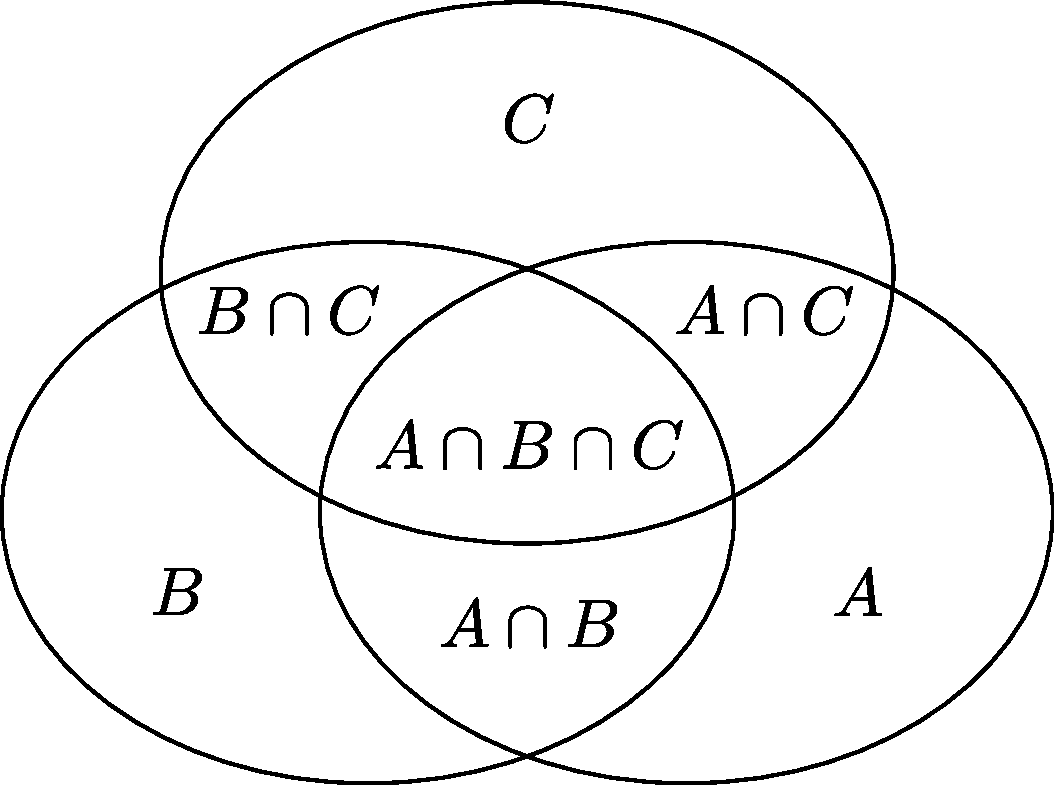
\includegraphics[angle=0, scale=0.22]{fig3.pdf}
\caption{\label{fig3}  Representação gráfica do conjunto $(A \cup B \cup C)$ para a verificação do princípio de inclusão-exclusão.}
\end{center}
\end{figure} 
Assim, 
$$
\begin{aligned}
|A \cup B \cup C| &= |A \cup (B \cup C)| \\
&= |A| + |B \cup C| - |A \cap (B \cup C)| \\
&= |A| + |B| + |C| - |B \cap C| - |(A \cap B) \cup (A \cap C)| \\
&= |A| + |B| + |C| - |B \cap C| - (|A \cap B| + |A \cap C| - |A \cap B \cap C|) \\
&= |A| + |B| + |C| - |A \cap B| - |A \cap C| - |B \cap C| + |A\cap  B \cap C|. \\
\end{aligned}
$$
O qual verifica a fórmula para $n=3.$
\end{frame}
%=====================================================================

%=====================================================================
\begin{frame}
\begin{exem}
Quantos são os números inteiros positivos menores que 504 e primos com 504? 
Usando a decomposição em fatores primos temos que $504 = 2^3 \times 3^2 \times 7.$ Agora, definimos os conjuntos 

$$
\begin{aligned}
A & = \{1, 2, \ldots , 504\},\\
A_1 &= \{x \in A : x \ \text{é múltiplo de} \ 2\},\\
A_2 &= \{x \in A : x \ \text{é múltiplo de} \ 3\}, \\
A_3 &= \{x \in A : x \ \text{é múltiplo de} \ 5\}. \\
\end{aligned}
$$
Desejamos calcular a cardinalidade do conjunto $A - (A_1 \cup A_2 \cup A_3 )$. Desta forma, 
$|A_1|= 504/2 = 252,$
$|A_2|= 504/3 = 168,$ 
$|A_3|= 504/7 = 72,$ 
$|A_1 \cap A_2 | = 504/ (2\times 3) = 84,$ 
$|A_1 \cap A_3| = 504/  (2\times 7) = 36,$ 
$|A_2 \cap A_3 | = 504/ (3\times 7)=  24,$  
$|A_1 \cap A_2 \cap A_3 | = 504/ (2\times 3\times 7)=  12. $ 
Usando o princípio de inclusão-exclusão
$$|A_1 \cup A_2 \cup A_3 | = 252 + 168 + 72 - 84 - 36 - 24 + 12 = 360.$$
Assim, existem ao todo 144 números inteiros positivos menores que 504 e primos com 504.
\end{exem}
\end{frame}
%=====================================================================




%=====================================================================
\begin{frame}{Variações com repetição: Amostras com ordem e com substituição.} Suponhamos que temos uma gaveta com $n$  objetos distintos. Desejamos realizar $k$ extrações ao acaso de um objeto ao mesmo tempo. Ao efetuar uma extração, registramos o objeto escolhido (marcamos o objeto, isto é o distinguimos) e o devolvemos à gaveta, desta forma o objeto pode ser selecionado várias vezes. Em cada extração temos $n$ objetos possíveis para serem escolhidos e efetuamos $k$ extrações. 

Assim pelo princípio da multiplicação o número total de arranjos que podem ser obtidos desta gaveta ao se fazer $k$ extrações é 
$$\displaystyle{\underbrace{n\cdot n\cdots n}_{\text{\normalsize $n$ vezes}}=n^k.}$$ 
Este número é chamado de {\it ordenações com repetição}. 

\begin{exem}
Suponhamos que temos um conjunto de 60 caracteres distintos. este conjunto contém todas as letras minúsculas e as letras maiúsculas do alfabeto, os dez dígitos e alguns caracteres especias como: $\%, @, \$, \#,$ etc. Quantas senhas de comprimento 6 podem ser construídas usando estes 60 caracteres?

Como cada caracter dos 60 disponíveis pode ser escolhido para ser colocado em cada uma das seis posições da senha, então podemos construir $60 \times 60 \times 60 \times 60 \times 60 \times 60= 60^6 =4.6656\times 10^{10} $ distintas senhas.
\end{exem}

 
\end{frame}
%=====================================================================

%=====================================================================
\begin{frame}{Variações sem repetição: Amostras com ordem e sem substituição.} Temos uma gaveta com $n$ objetos e dos quais se devem extrair, um a um $k$ objetos. Suponhamos que nesta situação a amostra é {\it sem substituição}, isto quer dizer, uma vez selecionado um  objeto este não é devolvido à gaveta. O total de arranjos distintos que podemos obter é 
\begin{equation}
\label{perm1}
n(n-1)(n-2)\cdots (n-k-1). 
\end{equation}
Pelo princípio da multiplicação notamos que há $k$ fatores na expressão anterior. O primeiro fator é $n$ e isto é devido ao fato que temos qualquer dos $n$ objetos para serem colocados na primeira posição, para a segunda posição temos $(n-1)$ objetos, para a terceira posição $(n-2)$ objetos, e assim por diante. este raciocínio termina ao escolher o $k$-ésimo objeto para o qual temos unicamente $(n-k+1)$ possibilidades. A expressão anterior pode ser escrita como 
$$
P(n,k) = \frac{n!}{(n-k)!}, \quad k \leq n
$$ 
e se chama de {\it permutação de $n$ em $k$}. 
 \begin{exem}
De quantas formas podem ser atribuídos ou primeiro, segundo e terceiro prêmio em uma rifa de 10 boletos numerados de 1 até 10? Notemos que de fato este problema é um problema de ordenação sem repetição de 10 objetos em que devem ser extraídos 3 objetos de estes. Daí, existem $10\times 9\times 8=720 $ distintas atribuições para os três primeiros números na rifa. 
\end{exem}

 
\end{frame}
%=====================================================================


%=====================================================================
\begin{frame}{Permutações: Amostras exaustivas com ordem e sem substituição.} A pergunta básica a respeito do número total de formas em que podemos colocar em um ordem linear (um  elemento após o outro e portanto sem repetição) $n$ objetos distintos tem com resposta o chamado {\it fatorial} de| $n,$ o qual é denotado por $$n! = n(n-1)(n-2)\cdots 3\cdot 2 \cdot 1.$$ Por definição temos que $0!=1.$

\begin{exem}
Suponhamos que queremos acomodar algumas crianças em uma fila, quatro meninas e três meninos. Se os meninos e meninas podem ser alocados em qualquer ordem então há $7!=5040$ formas de acomodar as crianças. Agora se queremos que os meninos e as meninas fiquem alternados na fila então há 
$(4\times 3) \times (3\times 2) \times (2\times 1) \times 1 = 144$ formas de organizá-los. Se desejamos que os meninos formem um grupo e as meninas formem outro grupo na fila temos $2\times 4! \times 3! =288$ formas de acomodá-los. 
\end{exem}

\end{frame}
%=====================================================================


%=====================================================================
\begin{frame}{Combinações: Amostras sem ordem e sem substituição} Suponhamos  que temos um conjunto de $n$ objetos distinguíveis e estamos interessados em obter uma amostra (subconjunto)  de tamanho $k.$ Suponhamos que as amostras agora devem ser {\it sem ordem e sem repetição}.  Lembremos que quando a ordem importa temos ${n!}/{(n-k)!}$ possibilidades. Agora, como não estamos interessados na ordem observamos que um dos arranjos desta fórmula está sendo contado $k!$ vezes. As vezes em que os mesmos $k$ elementos podem ser permutados uns com os outros, uma vez que o conjunto de dados é o mesmo. Assim, para obter arranjos em que a ordem não importa devemos então dividir por $k!.$ Está fórmula se chama de {\it combinações de $n$ em $k$} a qual é denotada por 
\begin{equation}
\label{comb}
    C_n^k = {n\choose k} = \frac{n!}{k!\cdot\left(n - k\right)!}, 
\end{equation}
em que  $n$ é o total de elementos e $k$ é o número de elementos escolhidos. 

Note que da equação \ref{comb} pode ser deduzido que 
\begin{equation}
\label{comb2}
{n \choose k} = {n \choose n-k} .
\end{equation}
De fato, se o número $\displaystyle{{n \choose k}}$ representa o número de subconjuntos de $k$ elementos
de um conjunto de $n$ elementos, então, se inicialmente escolhemos $k$ objetos estamos deixando de lado $n-k$ objetos, que é equivalente a escolher $n-k$ objetos que logo serão deixados de lado.
 
\end{frame}
%=====================================================================

%=====================================================================
\begin{frame}
\begin{exem}{Megassena}
Uma importante aplicação de combinação  é nas loterias:
Megassena, quina entre outras. A megassena consiste em uma cartela de 60
números dentre os quais devemos acertar 6 (prêmio principal). Calcule a
quantidade total de resultados possíveis para o prêmio principal.

Para marcar um cartão, precisamos escolher 6 entre 60 números, em que a
ordem de escolha não interfere no cartão que será marcado. Trata-se portanto, de
acordo com a definição, de um problema de combinação (devemos
combinar 60 números, em grupos de 6 números, ou seja, queremos subconjuntos
de 6 elementos de um conjunto de 10 elementos). O número de cartões é 
$$\displaystyle
{60 \choose 6} = 50063860
$$
 
\end{exem}

\begin{exem}
Seja $A$ um conjunto finito com $n$ elementos, então $A$ possui $2^n$ subconjuntos. De fato, sabemos que o coeficiente  
$\displaystyle{{n \choose k}}$ representa o número de subconjuntos de $k$ elementos de um conjunto de $n$ elementos. 
Então, se somamos em $k$ ($k=0$ elementos, $k=1$ elementos, e assim por diante ate $k=n$ elementos ) obtemos o número de subconjuntos do conjunto $A$. 
$$
{n \choose 0} + {n \choose 1} + {n \choose 2} + \cdots + {n \choose n} = (1+1)^n = 2^n.
$$
\end{exem}
 
\end{frame}
%=====================================================================


%=====================================================================
\begin{frame}
\begin{block}{Modelos de gavetas}
Suponhamos que em uma caixa há $N$ bolas do mesmo tipo, mas de cores diferentes, a saber: $R$ bolas
vermelhas e $N-R$ brancas. Se extraem ao  acaso $n$ bolas. Qual é  a probabilidade de extrair exatamente $k \leq n$ bolas vermelhas?

Suponhamos que as bolas se encontram  enumeradas de 1 até $N$ e que a enumeração das bolas vermelhas vá de 1 até $R$. Nesta situação devemos lembrar que é necessário distinguir dois casos. A extração é feita com substituição  e a  extração é feita sem substituição. No primeiro caso podemos considerar duas alternativas: 

\begin{enumerate}
\item[i)] As bolas são retiradas uma após a outra : As $n$ bolas são extraídas uma a uma da caixa e deixadas fora da caixa. Neste caso o espaço 
amostral está dado por:
$$\Omega= \{ (a_1, a_2, \dots \, , a_n): a_j \in \{1,2,\dots \, , N \} \, , a_i \not= a_j, i \not= j, j=1,2, \dots , n \}$$  
Então, definimos os eventos 
\begin{center}
$A_k$=``exatamente $k \leq n$ bolas vermelhas são extraídas''.
\end{center}
Note que $A_k$ é uma $n$-upla em $\Omega ,$ que contém exatamente $k$ componentes menores ou iguais a $R$. Temos desta forma que: 

\begin{equation*}\displaystyle
\begin{aligned}
\left| \Omega \right| &=  N(N-1)...(N-(n-1))=(N)_n \\
\left| A_k \right| &= \binom{n}{k} R(R-1) ... (R-k+1)(N-R)...(N-R-(n-k)+1) \\
&=\binom{n}{k}P(R,k) P(N-R, n-k). \\
\end{aligned}
\end{equation*}

\end{enumerate}

 \end{block}
\end{frame}
%=====================================================================

%=====================================================================
\begin{frame}
\begin{block}{}
 Agora, ao supormos que o experimento é Laplaciano, tem-se
\begin{equation*}
 P(A_k)=\frac{\left|A_k \right|}{ \left|\Omega\right|}= \displaystyle{\frac{\binom{R}{k} \binom{N-R}{n-k} }{ \binom{N}{n}}} .
\end{equation*}
\begin{enumerate}
\item[ii)] As bolas são todas retiradas ao mesmo tempo: As $n$ bolas são todas extraídas ao tempo; neste caso temos que 
$\Omega =\{T:T \subseteq\{1,2,\ldots,N \}, \text{com}  \left|T\right|=n\}$ e $A_k$ definido como em i) consta de
todos os subconjuntos de  $\{1,2,  \dots ,N\}$ que contém  exatamente $k$ componentes menores ou iguais a $R$. Desta
forma  $\left| \Omega\right|= \binom{N}{n} $  e $\left| A_k\right|= \binom{R}{k} \binom{N-R}{n-k}.$ Se supursemos novamente que o experimento é Laplaciano 
\begin{equation*} 
\displaystyle{P(A_k)=\frac{\binom{R}{k} \binom{N-R}{n-k} } { \binom{N}{n}}}.
\end{equation*}

Se unicamente interessa o número $k$ de bolas vermelhas entre as $n$
bolas extraídas da caixa, temos que
\begin{equation*} 
\displaystyle{p_k= \frac{\binom{R}{k} \binom{N-R}{n-k}}{
\binom{N}{n}}  , \quad k = 0,1,2, \dots , n}
\end{equation*} 
define uma medida de probabilidade sobre o conjunto $\Omega^\prime=\{0,1, \dots  , n\} $, chamada de \textit{distribuição
hipergeométrica} com parâmetros $n$, $R$ e $N$, a qual é denotada por $H_g (n,R,N)$. 
\end{enumerate}
\end{block}
\end{frame}
%=====================================================================

%=====================================================================
\begin{frame}
\begin{block}{}
 No segundo caso, a extração é com substituição, cada bola extraída  é devolvida imediatamente à caixa; depois de misturar as bolas, extrai-se aleatoriamente a seguinte bola e  assim por diante. Neste caso, temos que o espaço amostral é igual a: 
$$
\begin{aligned}
\Omega &= \{(a_1, a_2, \ldots \, , a_n) : a_j \in \{1,2, \dots , N\},\ j= 1,2, \dots , n\}\\
&=\{1,\dots , N\}\times \{1, \dots , N\}\times \cdots \times\{1, \dots , N\} \\ 
&=\{1, \dots , N\}^n,  
\end{aligned}
$$
e o evento $A_k$ consta de todos os elementos $ (a_1, a_2, \ldots \, , a_n) \in \Omega$ com exatamente 
$k$ componentes menores ou iguais a $R$. Temos assim, $ \left| \Omega \right| =  N\cdot N \, \cdots \, N=N^n$ e $$\left|A_k \right|=\binom{n}{k}R^k(N-R)^{n-k}. $$ Portanto, se supursemos que todas as bolas têm a mesma chance de serem extraídas, então 
$$P(A_k)=\binom{n}{k}\frac{R^k(N-R)^{n-k}}{N^n}=\binom{n}{k}p^k q^{n-k},$$ em que $p=R/N$ e $q=1-p.$ 
Se estamos interessados unicamente no número $k$ de bolas vermelhas entre as $n$ bolas extraídas,  temos que

$$p_k= \binom{n}{k}p^k q^{n-k}, \qquad k=0,1,2,\dots , n, \qquad 0<p<1, q=1-p$$ define una medida de probabilidade sobre o conjunto 
$\Omega^\prime =\{0,1,2, \dots ,n\}$  chamada de  \textit{distribuição binomial} com parâmetros $n$ e $p$ a qual é denotada por ${\cal B}(n,p).$ 
\end{block}
\end{frame}
%=====================================================================


%=====================================================================
\begin{frame}{Probabilidade condicional}
\vspace{1cm}
\begin{itemize}
 
\item A probabilidade é uma forma de quantificar a incerteza de um fenômeno. Naturalmente se obtemos mais informações sobre o fenômeno em estudo essa nova informação pode alterar,  e por vezes de forma muito significativa a avaliação da probabilidade. 


\item Desde o ponto de vista frequentista, seja $A$  um evento aleatório, cuja ``chance'' de acontecer deve ser medida sob a suposição de que um evento $B$ tenha sido observado. Suponhamos que o experimento é repetido $n$ vezes sob as mesmas condições. Então, a frequência relativa de $A$ sob a condição $B$ é definida como 
$$
fr(A|\,B)=\frac{|A \cap B|} {|B|} \ \ \text{se} \ \ |B| > 0 
$$
em que $|B|$ é o cardinal do conjunto $B$ e $|A \cap B |$ é o número de casos favoráveis (cardinal do conjunto) ao evento $(A \cap B).$ 

\item É evidente que  $fr(A|B)$ depende de $n$. Contudo, se o experimento foi  observado para $n$ suficientemente grande, as frequências relativas tendem a se estabilizar  ao redor de um valor específico entre 0 e 1. Este valor é conhecido como 
probabilidade condicional  de $A$ dado $B.$ 
\end{itemize}
\end{frame}
%=====================================================================

%=====================================================================
\begin{frame}
\begin{defi}[Probabilidade condicional]
Sejam $(\Omega , {\cal F},P)$ um espaço de probabilidade e $B \in {\cal F}$
tal que  $P(B)>0$. A \textit{probabilidade condicional de $A$ sob a condição $B$}, $P(A|B)$ é definida como sendo
$$P(A|B)=\frac{P(A \cap B)}{P(B)}.$$
\end{defi}

\begin{exem}
Se atiram dois dados honestos ao ar. Qual é a probabilidade condicional de que pelo menos um resultado seja 6 dado que as faces dos dados são diferentes? Para solucionar este problema note que $\Omega =\{(a,b):a,b\in \{1,2,\ldots ,6\}\}$ e definamos os eventos 
$$
\begin{aligned}
A &=\text{``Pelo menos um dado cai com a face igual a 6''} \\
B &=\text{``As faces dos dois dados são distintas''} \\
\end{aligned}
$$

Neste caso, 
$$
\begin{aligned}
A = &\{(1,6),(2,6),(3,6),(4,6),(5,6),(6,1),(6,2),(6,3),(6,4), (6,5),(6,6)\}, \\ 
B = &\{(a,b) \in \Omega\,:\,a  \neq  b\}.
\end{aligned}
$$
Assim,  $$P(A|B)=\frac{P(A\cap B)}{P(B)}=\frac{\frac{10}{36}}{\frac{30}{36}}= \frac{1}{3}.$$
\end{exem}

 
\end{frame}
%=====================================================================

%=====================================================================
\begin{frame}
 \begin{teo}[Medida de probabilidade condicional]
 Dado que $B$ occore, os eventos favoráveis as $A$ são aqueles que pertencem a $A\cap B.$ Assim, para $(\Omega ,{\cal F}, P)$ um espaço de probabilidade em que $B\in {\cal F}$ com $ P(B)>0$. Então:

\begin{enumerate}
\item[A.1]$P(A|B)\geq 0,$ para todo $ A\in {\cal F},$
\item[A.2] $P(\Omega|B)=1,$ (medida finita).
\item[A.3] ($\sigma$-aditividade) Se $A_1, A_2, \ldots$ é uma sequência de eventos de
${\cal F}$  mutuamente excludentes, i.e., $A_i\cap A_j=\emptyset$ para todo
$i\neq j,$ então 
$$
\displaystyle
\label{ax3}
P\left(\bigcup_{i=1}^\infty A_i \Big | B \right)=\sum_{i=1}^\infty P(A_i|B)
$$
\end{enumerate}
\end{teo}
\begin{block}{Outras propriedades}
\begin{itemize}

\item[i)]$P(\ \cdot \ |A)$ é uma medida de probabilidade sobre $\Omega $, que está 
``concentrada'' em $A$, isto quer dizer, $P(A|A)=1$.

\item[ii)] Se $A\cap B=\emptyset $, então  $P(B|A)=0.$

 \item[iii)] $P(B\cap C|A)=P(B|A\cap C)P(C|A)$ se $P(A \cap C)>0.$ 
% 
% \item[iv)] Sejam $A_{1},A_{2},\ldots ,A_{n}\subseteq \Omega $, então 
% $$
% \begin{aligned}
% &P( A_{1}\cap A_{2}\cap \ldots \cap A_{n})\\ & =P( A_{1}\,|A_{2}\cap A_{3}\cap
% \ldots \cap A_{n})P( A_{2}\,|A_{3}\cap A_{4}\cap \ldots \cap A_{n})\cdots P(A_{n-1}\,|A_{n})P(A_{n}),
% \end{aligned}
% $$
% sempre e quando as probabilidades envolvidas estejam bem definidas.
\end{itemize}
\end{block}

\end{frame}
%=====================================================================

%=====================================================================
\begin{frame}
 \begin{teo}[Regra da multiplicação]
Consideremos uma sequência finita de  eventos aleatórios $A_1, A_2,\ldots, A_n$ tais que os eventos condicionais $ A_i|A_1\cap A_2\cap\ldots\cap A_{i-1} $ tenham probabilidades positivas. Então temos que a probabilidade de acontecerem todos os eventos é 
\[P\left(\bigcap_{i=1}^nA_i\right)=P(A_1)P(A_2|A_1)P(A_3|A_1\cap A_2)\ldots P(A_n|\cap_{i=1}^{n-1}A_i).\] 	
\end{teo}

\begin{proof}\[P\left(\bigcap_{i=1}^nA_i\right)=P(A_1)\frac{P(A_1\cap A_2)}{P(A_1)}\frac{P(A_1\cap A_2\cap A_3)}{P(A_1\cap A_2)}\ldots \frac{P(\bigcap_{i=1}^n A_i)}{P(\bigcap_{i=1}^{n-1} A_i)},\] 	
e usando a definição de probabilidade condicional, podemos reescrever o lado direito da igualdade acima como
\[P(A_1)P(A_2|A_1)P(A_3|A_1\cap A_2)\ldots P(A_n|\cap_{i=1}^{n-1}A_i)\]
o qual verifica a regra. 	
\end{proof}

Como caso particular temos que para  dois eventos $A$ e $B$ a probabilidade de ocorrência simultânea destes dois eventos dado que ocorreu o evento $B$ (ou $A$) é 
% é igual a probabilidade de ocorrência do evento $A$ (ou $B$) vezes a probabilidade de ocorrência do evento $A$ (ou B) dado que ocorreu o evento $B$ (ou $A$), ou seja
\[P(A\cap B)=P(B)P(A|B).\]
\end{frame}
%=====================================================================

%=====================================================================
\begin{frame}
 \begin{exem}
Num jogo de cartas, três cartas, são retiradas sem substituição de um baralho (52
cartas). Qual a probabilidade de que nenhuma das cartas retiradas seja um ouro?
Note que qualquer carta tem a mesma probabilidade de ser retirada. Agora definamos  o evento 
$$A_i = \{ \text{a $i$-ésima carta não é ouro}\},$$ para $i = 1, 2, 3$. Desejamos obter 
obter $P(A_1\cap  A_2 \cap A_3)$. Lembremos que cada naipe possui 13 cartas. 
As probabilidades condicionais deste experimento são 
$$
\begin{aligned}
P(A_1) &=\frac{39}{52}, \\
P(A_2 | A_1) &= \frac{38}{51}, \\
P(A_3 | A_1 \cap  A_2) &= \frac{37}{50}.
\end{aligned}
$$
Logo, pela regra da multiplicação
$$P(A_1 \cap A_2 \cap A_3) =\frac{39}{52}\times\frac{38}{51}\times\frac{37}{50} \approx 0,41.$$
\end{exem}

\end{frame}
%=====================================================================

%=====================================================================
\begin{frame}
\begin{teo}[Teorema da probabilidade total] 
\label{teoBayes}
Sejam $A_1, A_2, \ldots, A_n$ eventos dois a dois disjuntos que formam uma partição do espaço amostral, isto é, $ \displaystyle \bigcup_{i=1}^nA_i=\Omega $ e assuma que $P(A_i) > 0$  para $i = 1, 2, \ldots, n.$ Então, para qualquer evento $B$, temos que

\[
\begin{aligned}
P(B)&=P(A_1\cap B) + \cdots + P( A_n \cap B) \\ &= P(A_1) P(B|A_1) + \cdots + P(A_n)P(B|A_n)= \displaystyle \sum_{i}P(A_i)P(B|A_i).
\end{aligned}
\] 	
\end{teo}
Uma representação esquemática do teorema anterior pode ser vista no gráfico da Figura \ref{fig5}.
\begin{figure}[!htb]
\begin{center}
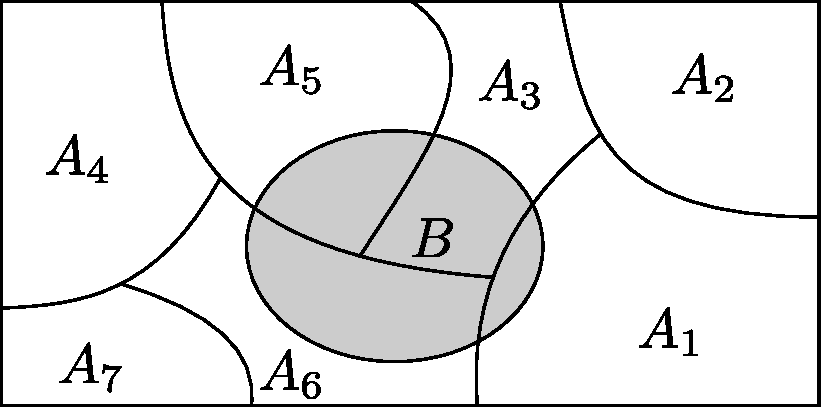
\includegraphics[angle=0, scale=0.4]{fig5.pdf}
\end{center}
\caption{\label{fig5}  Representação esquemática do teorema da probabilidade total para $n=7$.}
\end{figure} 
 
\end{frame}
%=====================================================================


%=====================================================================
\begin{frame}
 \begin{proof}
Para demonstrarmos o teorema anterior basta observarmos (ajudando pelo gráfico da Figura \ref{fig5}) que a sequência de eventos $ A_1, A_2, \ldots $ forma uma partição, então para qualquer $ B\subset \Omega $, segue que,  $ B=\displaystyle\bigcup_{i}(A_i\cap B) $ e como os $ A_i $ são disjuntos dois a dois temos que $ B\cap A_i $ também são disjuntos e pelo axioma 3 e pelo teorema anterior concluímos que
$$P(B)=\displaystyle \sum_{i}P(A_i\cap B)=\sum_{i}P(A_i)P(B|A_i).$$ 	
\end{proof}




Como corolário do teorema \ref{teoBayes} obtemos a muito famosa regra de Bayes, a qual constituí o alicerce da inferência Bayesiana. 

\begin{corol}[{\bf Teorema de Bayes ou regra de Bayes}] Seja $(\Omega ,{\cal F}, P)$ um espaço de probabilidade e $A_{1},A_{2},\ldots,$ uma partição 
finita de $\Omega$, então  é satisfeita para cada
$B\in {\cal F}$  com $P(B)>0$ a fórmula:
$$
P(A_{n}|B)=\frac{P(B|A_{n})P(A_{n})}{\sum_{j}P(B|A_{j})P(A_j)}, \quad \text{para todo} \quad  n.
$$
\end{corol}


\end{frame}
%=====================================================================

%=====================================================================
\begin{frame}
 \begin{proof}
$$P(A_{n}|B)=\frac{P(A_{n}\cap B)}{P(B)}=
\frac{P(B|A_{n})P(A_{n})}{\sum_{j}P(B|A_{j})P(A_{j})}.$$
\end{proof}
Para dar uma interpretação à regra de Bayes, suponhamos que os eventos $A_1, A_2, \ldots $ são todas as possíveis causas, mutuamente excludentes de um evento $B.$ Sob a suposição de que o evento $B$ tenha sido observado, a fórmula de Bayes permite conhecer qual dessas causas é a mais provável de haver produzido o evento $B.$

\begin{defi}[Distribuição a priori e a posteriori]
Seja $A_{1},A_{2},\ldots ,$ uma partição finita ou enumerável de $\Omega $, e seja $B \in {\cal F}$ com $P(B)>0$. Então 
$(P(A_{n}))_{n}$ é chamada  de \textit{distribuição ``a priori''}, isto é, antes de que aconteça $B.$ A probabilidade $(P(A_{n}|B))_{n}$ é chamada de 
\textit{distribuição ``a posteriori''}, isto significa, depois que aconteceu $B.$
\end{defi}

Uma possível e muito clara regra de decisão diante uma situação de interesse, digamos a presença do evento $B$ se considere como ocorrido o evento $A_n$ como aquele que tem a maior probabilidade sob a hipótese de que o evento $B$ acontece, portanto, elege-se entre os possíveis eventos $A_n$ aquele que dando por acontecido $B$ tem a maior probabilidade de ocorrer. Naturalmente, esta decisão não está eximida de erro, mas pode ajudar a indicar a probabilidade de uma decisão falsa.
\end{frame}
%=====================================================================

%=====================================================================
\begin{frame}
\begin{exem}
Numa determinada cidade são feitos testes para detectar uma determinada doença. Suponhamos que  1\% das pessoas sadias são registradas como doentes,  0,1\% da população está realmente doente e  90\% dos doentes são de fato registrados como doentes. Qual é a probabilidade de que um cidadão seja registrado como doente? Qual é a probabilidade de que uma pessoa registrada como doente esteja  realmente doente?  
 \end{exem}
 
 Definamos os seguintes eventos $S$= ``sadio'', $E$= ``realmente doente'' e $T$=``registrado como doente''.  Então $P(T|\,S)=0.01$ e $P(T|\,E)=0,9$. Assim,  $$P(T)=P(T\cap (S{\huge \cup} E))=P(T|\,S)P(S)+P(T|\,E)P(E)=0,01\times 0,999+0.9\times 0,001\approx 0,01$$ e $$P(E|\,T)=P(T|\,E)P(E)/P(T)\approx 0,083.$$ Com estes resultados deduz-se que para este exemplo,  as distribuições a priori  e as distribuições a posteriori são respectivamente, (0,001, 0,999) e  (0,083, 0,917). 
\end{frame}
%=====================================================================

%%=====================================================================
%\begin{frame}
%\begin{exem}
%Um curso de economia possui três disciplinas de probabilidade obrigatórias (Prob I, II e III) no núcleo básico. Na primeira disciplina há 50\% dos estudantes, na segunda há 25\% dos estudantes e na terceira há 25\% dos estudantes. Todos eles pertencendo ao núcleo básico. As mulheres (M) se encontram distribuídas uniformemente, sendo que elas constituem  60\% dos alunos do núcleo básico. No gráfico da Figura \ref{arvore} estão representadas as probabilidades para este exemplo.
%\end{exem}
%
%
%
%% Set the overall layout of the tree
%\tikzstyle{level 1}=[level distance=3cm, sibling distance=1.5cm]
%\tikzstyle{level 2}=[level distance=3cm, sibling distance=1cm]
%
%% Define styles for bags and leafs
%\tikzstyle{bag} = [circle, text width=4em, text centered]
%\tikzstyle{end} = [minimum width=4pt,fill, inner sep=0pt]
%
%
%\begin{figure}[!htbp]
%\begin{center}
%{\footnotesize
%
%% The sloped option gives rotated edge labels. Personally
%% I find sloped labels a bit difficult to read. Remove the sloped options
%% to get horizontal labels. 
%\begin{tikzpicture}[grow=right, sloped]
%
%
%\node[bag] { Cursos}
%    child {
%        node[bag] {Alunos}        
%            child {
%                node[end] {}
%                edge from parent
%                node[above] {M}
%                node[below]  {$P(M | $Prob III $)=$ 0,6}
%            }
%            child {
%                node[end] {}
%                edge from parent
%                node[above] {H}
%                node[below]  {$P(H | $Prob III $)=$ 0,4}
%            }
%            edge from parent 
%            node[above] {Prob III}
%            node[below]  {$P($Prob III $)=$ 0,25}
%    }
%    child {
%        node[bag] {Alunos}        
%        child {
%                node[end] {}
%                edge from parent
%                node[above] {M}
%                node[below]  {$P(M | $Prob II $)=$ 0,6}
%            }
%            child {
%                node[end] {}
%                edge from parent
%                node[above] {H}
%                node[below]  {$P(H | $Prob II $)=$ 0,4}
%            }
%        edge from parent         
%            node[above] { \ \ Prob II}
%            node[below]  {$P($Prob II $)=$ 0,25}
%    }
%    child {
%        node[bag] {Alunos}        
%            child {
%                node[end] {}
%                edge from parent
%                node[above] {M}
%                node[below]  {$P(M | $Prob I $)=$ 0,6}
%            }
%            child {
%                node[end] {}
%                edge from parent
%                node[above] {H}
%                node[below]  {$P(H | $Prob I $)=$0,4}
%            }
%            edge from parent 
%            node[above] {Prob I}
%            node[below]  {$P($Prob I $)=$ 0,50}
%    }
%%\caption{Diagrama de árvore para o exemplo das disciplinas.}
%;
%%
%\end{tikzpicture}
%\caption{\label{arvore} Diagrama de árvore para o exemplo das disciplinas de probabilidade.}
%}
%\end{center}
%
%\end{figure}
%\end{frame}
%%=====================================================================

%=====================================================================
\begin{frame}{Independência de eventos}

Em algumas situações a ocorrência de um evento $B$ não afeta a ocorrência de um evento $A$ isto é, $P(A|B) = P(A)$ e neste caso dizemos que o evento $A$ é ``independente'' do evento $B.$ Contudo, está definição é válida unicamente se $P(B)>0.$ %Para contornar esta situação se assume a seguinte definição de independência  


\begin{defi}
Dois eventos $A$ e $B$ são ditos \textit{independentes} se 
$$P(A\cap B)=P(A)P(B).$$ Em caso contrário se diz que os eventos são dependentes.
\end{defi}


\begin{exem}
Um dado honesto é atirado ao ar duas vezes consecutivas.  Definamos os eventos $A= \ $ ``a soma dos resultados obtidos é um número par'' e $B= \ $ `` o segundo lançamento resulta ser um n\'{u}mero par''. Para este caso temos que $P(A)=P(B)=1/2$ e $P(A\cap B)=1/4$. Portanto $A$ e $B$ são eventos independentes. 
\end{exem}

\begin{exem}
Consideremos novamente o lançamento dos dados. Mas agora carregamos o dado de tal maneira que a probabilidade de obter um n\'{u}mero par é 2/5. Se consideramos os eventos do exemplo anterior temos que $P(B)=2/5,$   $P(A)=13/25$ e $P(A\cap B)=4/25$.  Assim, $A$ e $B$ não são independentes.
\end{exem}
 
\end{frame}
%=====================================================================


%=====================================================================
\begin{frame}
%\vspace{-0.5cm}
\begin{defi}
Os $n$ eventos $A_{1},A_{2},\ldots ,A_{n}$ são 
ditos \textit{(completamente) independentes} se para todo $1\leq
j_{1}\leq j_{2}\leq \cdots \leq j_{k}\leq n$, $2\leq k\leq n$ satisfaz-se 
$$P(A_{j_{1}}\cap A_{j_{2}}\cap \ldots \cap A_{j_{k}})=P(
A_{_{j_{1}}})\cdots P(A_{_{j_{k}}}).$$
\end{defi}

Se segue da definição que:
\begin{enumerate}
\item[(1)] $P(A_{1}\cap A_{2}\cap \ldots \cap A_{n})=P($ $A_{1})P(A_{2})\cdots
P(A_{n}).$ 
\item[(2)] $P(A_{i}\cap A_{j})=P($ $A_{i})P(A_{j})$ \ para todo $i\neq j$.
\end{enumerate}
Note que nem (1) nem (2) sozinhas  implicam a independência dos eventos $A_{1},A_{2},\ldots ,A_{n}$ para o caso $n>2$. Ainda mais, o fato de que 
(1) e (2) sejam satisfeitos não implicam na independência total de $A_{1},A_{2},\ldots ,A_{n}$  para o caso $n>3$, como o ilustramos no seguinte exemplo:


\begin{exem}
Consideremos os seguintes eventos relacionados com o lançamento de um dado corrente duas vezes consecutivas. Definamos os eventos  
$A = \text{`` no primero lançamento é obtido um dois''}, $ $B =\text{`` no segundo lançamento é obtido um cinco''}$ e 
$C =$ {`` a soma dos resultados em ambos os lançamentos é sete ''}.

Neste caso, $P(A)=P(B)=P(C)=1/6$. Por outro lado, $P(A\cap B)=P(A\cap C)=P(B\cap C)=P((2,5))=1/36$. Portanto, satisfaz-se que 
$P(A\cap B)=P(A)P(B),$ $P(A\cap C)=P(A)P(C)$ e $P(B\cap C)=P(B)P(C).$ Contudo $$P(A\cap B\cap C)=P((2,5))\neq P(A)P(B)P(C).$$
\end{exem}
 
\end{frame}
%=====================================================================


%=====================================================================
\begin{frame}
 \begin{defi}[Probabilidade Geométrica]  Seja $(\Omega ,{\cal F}, P)$ um espaço de probabilidade e  $A \in {\cal F}$ um evento aleatório. Suponhamos que sobre $(\Omega ,{\cal F})$ seja definida uma medida geométrica $\mu$ tal como o comprimento, a área, o volume, etc. Definimos a probabilidade do evento $A$ como 
\begin{equation}
\label{pgeo}
P(A) = \frac{\mu(A)}{\mu(\Omega)}.
\end{equation}
\end{defi}

\begin{exem}[O jogo do ladrilho ] 
Uma moeda de raio $r$ é lançada ao acaso no chão o qual é coberto por
ladrilhos quadrados de lado $l$ $(l > 2r)$ como descrito na Figura \ref{fig7}. As crianças francesas no século XVIII apostavam que a moeda
cairia inteiramente dentro de um ladrilho. 

Buffon observou, que a probabilidade de a moeda cair inteiramente dentro
de um ladrilho era a probabilidade do centro da moeda cair dentro de um
quadrado de lado $l - 2r$. Essa probabilidade é a razão entre as áreas do quadrado e do ladrilho,
pois a probabilidade do centro da moeda cair em uma região é proporcional
à área dessa região.


\end{exem}
\end{frame}
%=====================================================================

%=====================================================================
\begin{frame}

\begin{figure}[!htb]
\begin{center}
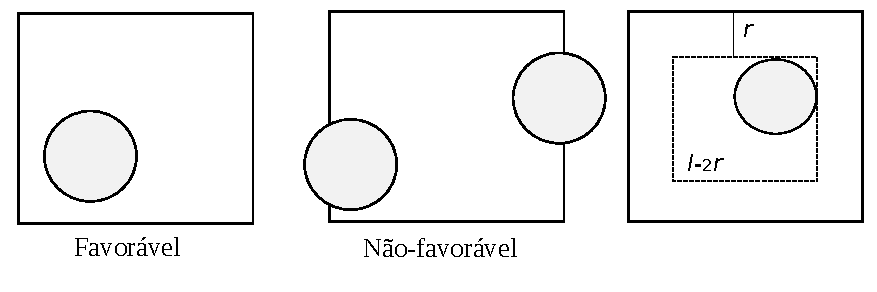
\includegraphics[angle=0, scale=0.5]{fig7.pdf}
\end{center}
\caption{\label{fig7} Representação esquemática do jogo dos ladrilhos.
}
\end{figure} 
  Portanto, a probabilidade da moeda cair inteiramente
dentro de um ladrilho é $$ \frac{( l-2r )^2}{l^2}.$$
Se consideramos um piso formado por quadrados de cerâmica de 30 cm de lado e um disco (``moeda'') de raio 5 cm, a probabilidade do disco cair inteiramente dentro de um dos ladrilhos é igual a $(30-10)^2/ 30^2 = 0,4444$ ou 44,44\%.


Nessa situação, o diâmetro $d$ do disco que daria 60\% de chances de vitória ao jogador é $d$ = 6,77 cm.
\end{frame}
%=====================================================================
% % 
% % %=====================================================================
% % \begin{frame}
% %  
% % \end{frame}
% % %=====================================================================
% % 
% % %=====================================================================
% % \begin{frame}
% %  
% % \end{frame}
% % %=====================================================================
% % 
% % 
% % %=====================================================================
% % \begin{frame}
% %  
% % \end{frame}
% % %=====================================================================
% % 
% % 
% % %=====================================================================
% % \begin{frame}
% %  
% % \end{frame}
% % %=====================================================================
% % 
% % %=====================================================================
% % \begin{frame}
% %  
% % \end{frame}
% % %=====================================================================
% % 
% % %=====================================================================
% % \begin{frame}
% %  
% % \end{frame}
% % %=====================================================================
% % 
% % %=====================================================================
% % \begin{frame}
% %  
% % \end{frame}
% % %=====================================================================
% % 
% % 
% % %=====================================================================
% % \begin{frame}
% %  
% % \end{frame}
% % %=====================================================================
% % 
% % 
% % %=====================================================================
% % \begin{frame}
% %  
% % \end{frame}
% % %=====================================================================
% % 
% % %=====================================================================
% % \begin{frame}
% %  
% % \end{frame}
% % %=====================================================================
\end{document}

